\documentclass[11pt,compress,t,notes=noshow, xcolor=table]{beamer}
\usepackage[]{graphicx}\usepackage[]{color}
% maxwidth is the original width if it is less than linewidth
% otherwise use linewidth (to make sure the graphics do not exceed the margin)
\makeatletter
\def\maxwidth{ %
  \ifdim\Gin@nat@width>\linewidth
    \linewidth
  \else
    \Gin@nat@width
  \fi
}
\makeatother

\definecolor{fgcolor}{rgb}{0.345, 0.345, 0.345}
\newcommand{\hlnum}[1]{\textcolor[rgb]{0.686,0.059,0.569}{#1}}%
\newcommand{\hlstr}[1]{\textcolor[rgb]{0.192,0.494,0.8}{#1}}%
\newcommand{\hlcom}[1]{\textcolor[rgb]{0.678,0.584,0.686}{\textit{#1}}}%
\newcommand{\hlopt}[1]{\textcolor[rgb]{0,0,0}{#1}}%
\newcommand{\hlstd}[1]{\textcolor[rgb]{0.345,0.345,0.345}{#1}}%
\newcommand{\hlkwa}[1]{\textcolor[rgb]{0.161,0.373,0.58}{\textbf{#1}}}%
\newcommand{\hlkwb}[1]{\textcolor[rgb]{0.69,0.353,0.396}{#1}}%
\newcommand{\hlkwc}[1]{\textcolor[rgb]{0.333,0.667,0.333}{#1}}%
\newcommand{\hlkwd}[1]{\textcolor[rgb]{0.737,0.353,0.396}{\textbf{#1}}}%
\let\hlipl\hlkwb

\usepackage{framed}
\makeatletter
\newenvironment{kframe}{%
 \def\at@end@of@kframe{}%
 \ifinner\ifhmode%
  \def\at@end@of@kframe{\end{minipage}}%
  \begin{minipage}{\columnwidth}%
 \fi\fi%
 \def\FrameCommand##1{\hskip\@totalleftmargin \hskip-\fboxsep
 \colorbox{shadecolor}{##1}\hskip-\fboxsep
     % There is no \\@totalrightmargin, so:
     \hskip-\linewidth \hskip-\@totalleftmargin \hskip\columnwidth}%
 \MakeFramed {\advance\hsize-\width
   \@totalleftmargin\z@ \linewidth\hsize
   \@setminipage}}%
 {\par\unskip\endMakeFramed%
 \at@end@of@kframe}
\makeatother

\definecolor{shadecolor}{rgb}{.97, .97, .97}
\definecolor{messagecolor}{rgb}{0, 0, 0}
\definecolor{warningcolor}{rgb}{1, 0, 1}
\definecolor{errorcolor}{rgb}{1, 0, 0}
\newenvironment{knitrout}{}{} % an empty environment to be redefined in TeX

\usepackage{alltt}
\newcommand{\SweaveOpts}[1]{}  % do not interfere with LaTeX
\newcommand{\SweaveInput}[1]{} % because they are not real TeX commands
\newcommand{\Sexpr}[1]{}       % will only be parsed by R
\newcommand{\xmark}{\ding{55}}%


\usepackage[english]{babel}
\usepackage[utf8]{inputenc}

\usepackage{dsfont}
\usepackage{verbatim}
\usepackage{amsmath}
\usepackage{amsfonts}
\usepackage{amssymb}
\usepackage{bm}
\usepackage{csquotes}
\usepackage{multirow}
\usepackage{longtable}
\usepackage{booktabs}
\usepackage{enumerate}
\usepackage[absolute,overlay]{textpos}
\usepackage{psfrag}
\usepackage{algorithm}
\usepackage{algpseudocode}
\usepackage{eqnarray}
\usepackage{arydshln}
\usepackage{tabularx}
\usepackage{placeins}
\usepackage{tikz}
\usepackage{setspace}
\usepackage{colortbl}
\usepackage{mathtools}
\usepackage{wrapfig}
\usepackage{bm}
\usepackage{amsmath}
\usepackage{pifont}
\usepackage{xcolor} %colored math symbols

\usetikzlibrary{shapes,arrows,automata,positioning,calc,chains,trees, shadows}
\tikzset{
  %Define standard arrow tip
  >=stealth',
  %Define style for boxes
  punkt/.style={
    rectangle,
    rounded corners,
    draw=black, very thick,
    text width=6.5em,
    minimum height=2em,
    text centered},
  % Define arrow style
  pil/.style={
    ->,
    thick,
    shorten <=2pt,
    shorten >=2pt,}
}

\usepackage{subfig}

% Defines macros and environments
\usepackage{../../style/lmu-lecture}


\let\code=\texttt
\let\proglang=\textsf

\setkeys{Gin}{width=0.9\textwidth}

\setbeamertemplate{frametitle}{\expandafter\uppercase\expandafter\insertframetitle}

\usepackage{bbm}
% basic latex stuff
\newcommand{\pkg}[1]{{\fontseries{b}\selectfont #1}} %fontstyle for R packages
\newcommand{\lz}{\vspace{0.5cm}} %vertical space
\newcommand{\dlz}{\vspace{1cm}} %double vertical space
\newcommand{\oneliner}[1] % Oneliner for important statements
{\begin{block}{}\begin{center}\begin{Large}#1\end{Large}\end{center}\end{block}}


%new environments
\newenvironment{vbframe}  %frame with breaks and verbatim
{
 \begin{frame}[containsverbatim,allowframebreaks]
}
{
\end{frame}
}

\newenvironment{vframe}  %frame with verbatim without breaks (to avoid numbering one slided frames)
{
 \begin{frame}[containsverbatim]
}
{
\end{frame}
}

\newenvironment{blocki}[1]   % itemize block
{
 \begin{block}{#1}\begin{itemize}
}
{
\end{itemize}\end{block}
}

\newenvironment{fragileframe}[2]{  %fragile frame with framebreaks
\begin{frame}[allowframebreaks, fragile, environment = fragileframe]
\frametitle{#1}
#2}
{\end{frame}}


\newcommand{\myframe}[2]{  %short for frame with framebreaks
\begin{frame}[allowframebreaks]
\frametitle{#1}
#2
\end{frame}}

\newcommand{\remark}[1]{
  \textbf{Remark:} #1
}


\newenvironment{deleteframe}
{
\begingroup
\usebackgroundtemplate{
\includegraphics[width=\paperwidth,height=\paperheight]{../style/color/red.png}}
 \begin{frame}
}
{
\end{frame}
\endgroup
}
\newenvironment{simplifyframe}
{
\begingroup
\usebackgroundtemplate{
\includegraphics[width=\paperwidth,height=\paperheight]{../style/color/yellow.png}}
 \begin{frame}
}
{
\end{frame}
\endgroup
}\newenvironment{draftframe}
{
\begingroup
\usebackgroundtemplate{
\includegraphics[width=\paperwidth,height=\paperheight]{../style/color/green.jpg}}
 \begin{frame}
}
{
\end{frame}
\endgroup
}
% https://tex.stackexchange.com/a/261480: textcolor that works in mathmode
\makeatletter
\renewcommand*{\@textcolor}[3]{%
  \protect\leavevmode
  \begingroup
    \color#1{#2}#3%
  \endgroup
}
\makeatother


\input{../../latex-math/basic-math}
\input{../../latex-math/basic-ml}
\input{../../latex-math/ml-nn}

\title{Deep Learning}

\date{}

\begin{document}
\newcommand{\titlefigure}{plots/GAN01.png}
%modify picture
\newcommand{\learninggoals}{
  \item architecture of a GAN
  \item minimax loss
  \item training a GAN
  %\item adversarial training 
  %\item projected gradient descent
  %\item fast gradient sign method
  %\item Principal component analysis
}


\lecturechapter{Introduction to Generative Adversarial Networks (GANs)}
\lecture{I2DL}


%\begin{frame} {Generative Adversarial Networks (GANs)}
%
%Generative adversarial networks
%\begin{itemize}
%\item define the generative model as in VAEs,
%\item but approach problem of learning a directed generative model $p(\mathbf{x}| \mathbf{z})$ from a totally different perspective.
%\vspace{1mm}
%\end{itemize}
%\begin{figure}
%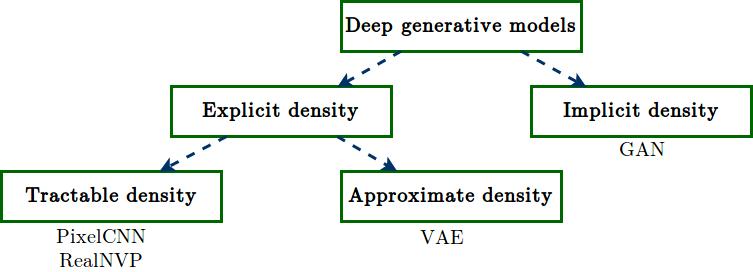
\includegraphics[width=8cm]{plots/taxonomy.png}
%\tiny{\\Taxonomy of Generative Model}
%\end{figure}

%\end{frame}

\begin{frame} {What is a GAN?}
    \begin{figure}
    \centering
    \scalebox{0.52}{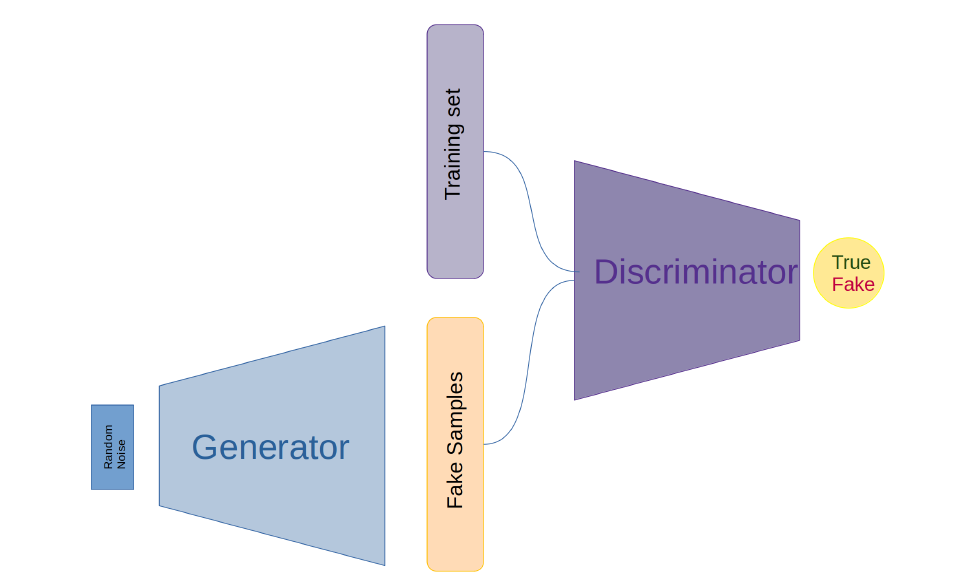
\includegraphics{plots/GAN01.png}}
    \end{figure}
    \begin{itemize}
    \item A  \emph{generative adversarial network} (GAN)  consists of two DNNs:
    \begin{itemize}
    \item generator 
    \item discriminator
    \end{itemize}
    \item Generator transforms random noise vector into fake sample. %in a given domain.
    \item Discriminator gets real and fake samples  as input and outputs %a number between 0 and 1 indicating the 
    probability of the input being real.
    \end{itemize}
    \end{frame}
    
    \begin{frame} {What Is a GAN?}
\begin{figure}
\centering
\scalebox{0.4}{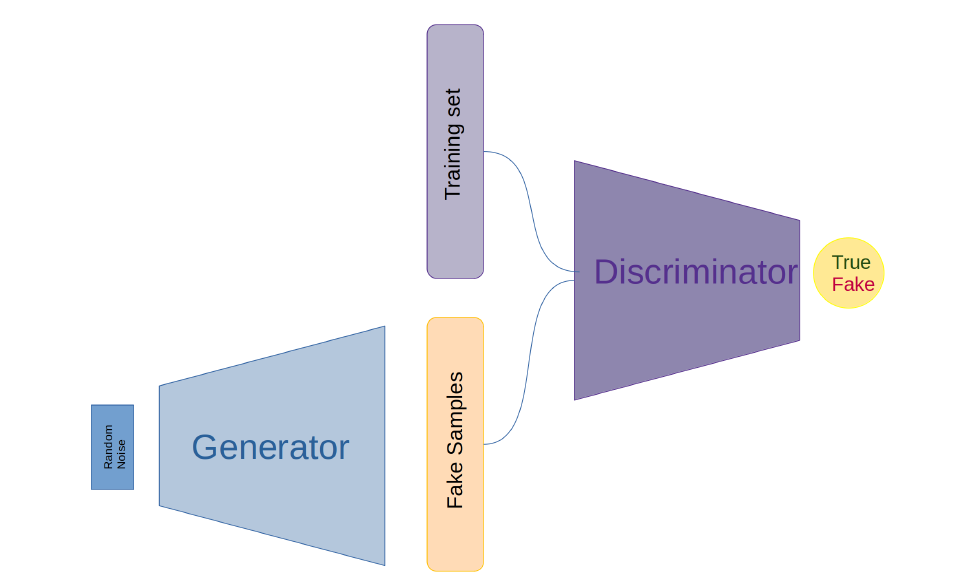
\includegraphics{plots/GAN01.png}}
\end{figure}
\begin{itemize}
\item Goal of generator: fool discriminator into thinking that the synthesized samples are real.
\item Goal of discriminator: recognize real samples and not being fooled by  generator.
\item This sets off an arms race. As the generator gets better at producing realistic samples, the discriminator is forced to get better at detecting the fake samples which in turn forces the generator to get even better at producing realistic samples and so on.
\end{itemize}
\end{frame}

\begin{frame} {Fake currency illustration}
\vspace{1mm}
The generative model can be thought of as analogous to a team of counterfeiters, trying to produce fake currency and use it without detection, while the discriminative model is analogous to the police, trying to detect the counterfeit currency. Competition in this game drives both teams to improve their methods until the counterfeits are indistinguishable from the genuine articles. \\
\hspace{45mm} -Ian Goodfellow

\begin{figure}
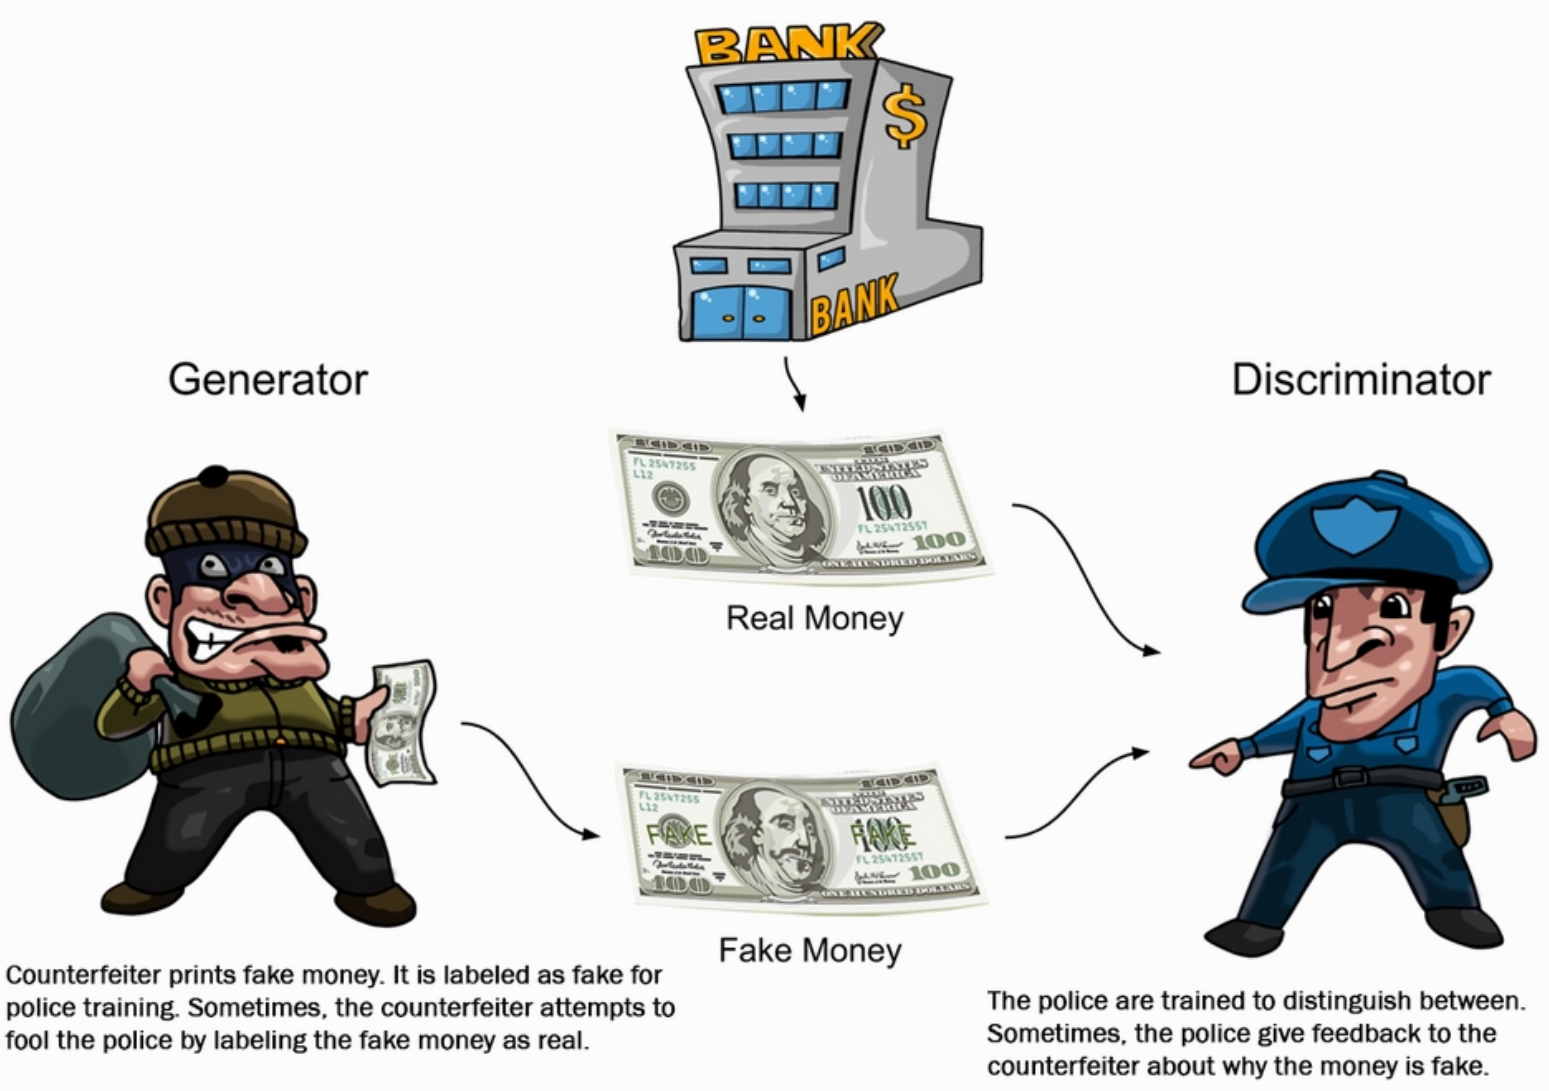
\includegraphics[width=5cm]{plots/counterfeiters.png}
\tiny{\\Image created by Mayank Vadsola}
\end{figure}

\end{frame}



\section{GAN Training}

\begin{frame} {Minimax Loss for GANs}
  \begin{tcolorbox}
  $\min \limits_G \max \limits_D V(D,G) = \E_{\mathbf{x}\sim p_{\text{data}(\mathbf{x})}}[\log D(\mathbf{x})] + \E_{\mathbf{z}\sim p(\mathbf{z})}[\log (1 - D(G(\mathbf{z})))]$
  \end{tcolorbox}
   \begin{itemize}
  \vspace{6mm}
      \item $p_{\text{data}(\mathbf{x})}$ is our target, the data distribution.
  \vspace{6mm}
  \item The generator is a neural network mapping a latend random vector $\mathbf{z}$ to generated sample $G(\mathbf{z})$. Even if the generator is a determinisic function, we have random outputs, i.e.~variability. 
      %\item Because a neural network (the generator) is a deterministic function, we feed a latent random vector $\mathbf{z}$ to the generator to induce variability in its outputs.
  \vspace{6mm}
      \item $p(\mathbf{z})$ is usually a uniform distribution or an isotropic Gaussian. It is typically fixed and not adapted during training.

   \end{itemize}
\end{frame}

\begin{frame} {Minimax Loss for GANs}
  \begin{tcolorbox}
    $\min \limits_G \max \limits_D V(D,G) = \E_{\mathbf{x}\sim p_{\text{data}(\mathbf{x})}}[\log D(\mathbf{x})] + \E_{\mathbf{z}\sim p(\mathbf{z})}[\log (1 - D(G(\mathbf{z})))]$
  \end{tcolorbox}
  \begin{itemize}
  \vspace{6mm}
    \item $G(\mathbf{z})$ is the output of the generator for a given state $\mathbf{z}$ of the latent variables.
  \vspace{6mm}
      \item $D(\mathbf{x})$ is the output of the discriminator for a real sample $\mathbf{x}$.
  \vspace{6mm}
      \item $D(G(\mathbf{z}))$ is the output of the discriminator for a fake sample $G(\mathbf{z})$ synthesized by the generator.
  \end{itemize}
\end{frame}


\begin{frame} {Minimax Loss for GANs}
  \begin{tcolorbox}
    $\min \limits_G \max \limits_D V(D,G) = \E_{\mathbf{x}\sim p_{\text{data}(\mathbf{x})}}[\log D(\mathbf{x})] + \E_{\mathbf{z}\sim p(\mathbf{z})}[\log (1 - D(G(\mathbf{z})))]$
  \end{tcolorbox}
  \begin{itemize}
    \item $\E_{\mathbf{x}\sim p_{\text{data}(\mathbf{x})}}[\log D(\mathbf{x})]$ is the log-probability of correctly classifying real data points as real. 
  \vspace{2mm}
    \item $\E_{\mathbf{z}\sim p(\mathbf{z})}[\log (1 - D(G(\mathbf{z})))]$ is the log-probability of correctly classifying fake samples as fake.
  \vspace{2mm}
    \item With each gradient update, the discriminator tries to push $D(\mathbf{x})$ toward 1 and $D(G(\mathbf{z})))$ toward 0. This is the same as maximizing V(D,G).
  \vspace{2mm}
    \item The generator  only has control over $D(G(\mathbf{z}))$ and tries to push that toward 1 with each gradient update. This is the same as minimizing V(D,G).
  \end{itemize}
\end{frame}

\begin{frame} {GAN training : Pseudocode}
  \begin{algorithm}[H]
  \footnotesize
    \caption{Minibatch stochastic gradient descent training of GANs. Amount of training iterations, amount of discriminator updates $k$ }
    \begin{algorithmic}[1]
      \For{number of training iterations}
        \For{k steps}
          \State Sample minibatch of $m$ samples $\{\mathbf{z}^{(1)} \ldots \mathbf{z}^{(m)}$\} from  prior $p_g(\mathbf{z})$
          \State Sample minibatch of $m$ examples $\{\mathbf{x}^{(1)} \ldots \mathbf{x}^{(m)}$\} from  training data 
 %generating distribution $p_{\text{data}}(\mathbf{x})$.
          \State Update discriminator by ascending the stochastic gradient: \item[]
  \hspace{2.5 cm}          $\nabla_{{\theta}_d} \frac {1}{m} \sum \limits_{i=1} \limits^{m} \left [ \log D(\mathbf{x}^{(i)}) + \log (1 - D(G(\mathbf{z}^{(i)}))) \right]$
            % + \log (1 - D(G(\mathbf{z}^{(i)})))}\right]$
        \EndFor
        \State Sample minibatch of $m$ noise samples $\{\mathbf{z}^{(1)} \ldots \mathbf{z}^{(m)}$\} from the noise prior $p_g(\mathbf{z})$
        \State Update generator by descending the stochastic gradient: \item[]
   \hspace{2.5 cm}       $\nabla_{{\theta}_g} \frac {1}{m} \sum \limits_{i=1} \limits^{m} \log (1 - D(G(\mathbf{z}^{(i)})))$
      \EndFor
    \end{algorithmic}
  \end{algorithm}
\end{frame}


\begin{frame} {GAN training: Illustration}
\begin{figure}
\centering
\scalebox{0.75}{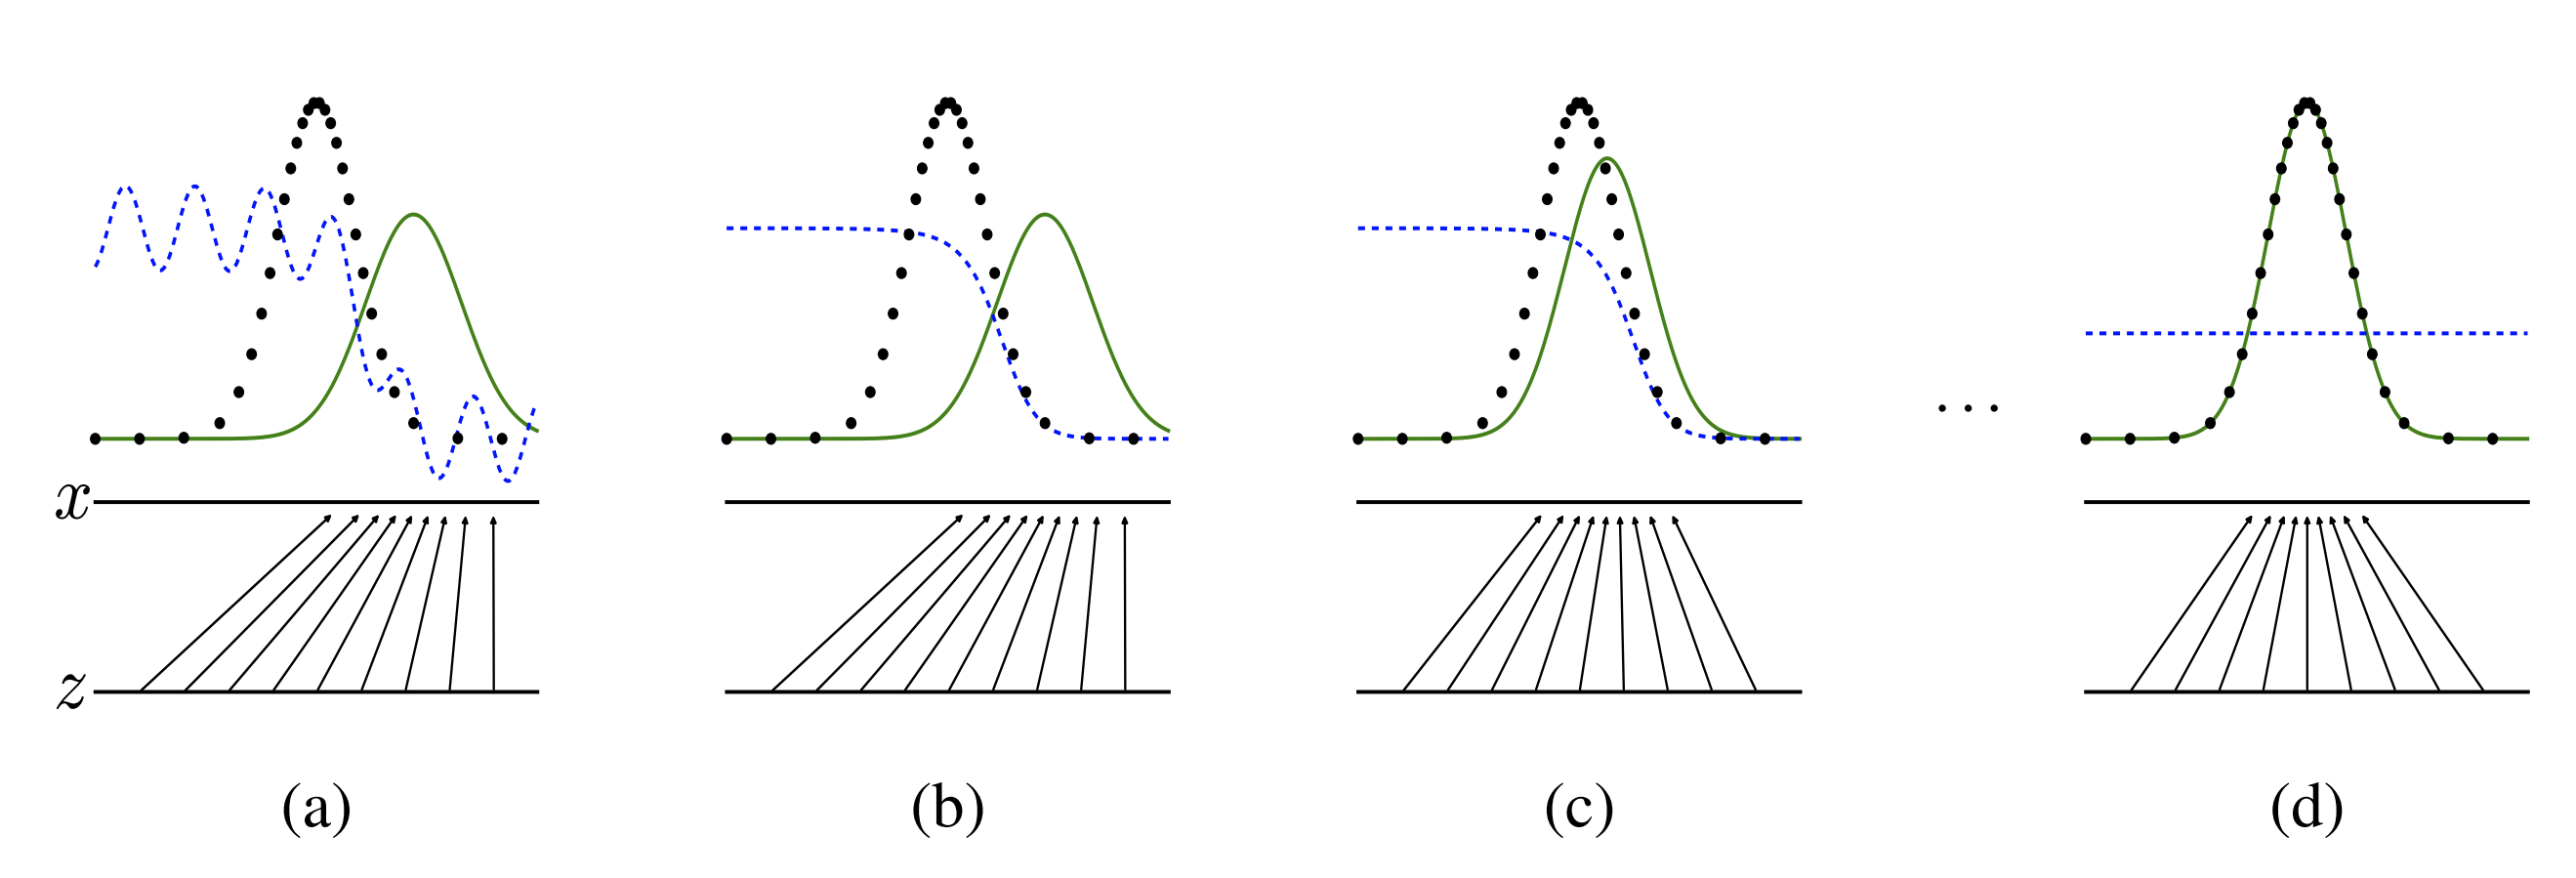
\includegraphics{plots/trainingGAN.png}}
\tiny{\\GANs are trained by simultaneously updating the discriminative distribution
(D, blue, dashed line) so that it discriminates between samples from the data generating distribution (black,dotted line) $p_x$ from those of the generative distribution $p_g (G)$ (green, solid line).Source: Goodfellow et al (2017),}
\end{figure}
\begin{itemize}
\item For $k$ steps, G's parameters are frozen and one performs \textbf{gradient ascent} on D to increase its accuracy.
\item Finally, D's parameters are frozen and one performs \textbf{gradient descent} on G to increase its generation performance. %/ to make D misclassify.
\item Note, that G gets to peek at D's internals (from the back-propagated errors) but D  does not get to peek at G.
\end{itemize}
\end{frame}

\begin{frame} {Divergence measures}
  \begin{itemize}
    \item The goal of generative modeling is to learn $p_{\text{data}}(\mathbf{x})$.
    \vspace{2mm}
    \item The differences between different generative models can be measured in terms of \textbf{divergence measures}.
    \vspace{2mm}
    \item A divergence measure quantifies the distance between two distributions. %It is a measure of how different one distribution is from another.
    \vspace{2mm}
    \item There are many different divergence measures that one can us (e.g. Kullback-Leibler divergence).
    \vspace{2mm}
    \item All such measures always  positive and  0 if and only if the two distributions are equal to each other.
  \end{itemize}
\end{frame}

\begin{frame} {Divergence measures}
  \begin{itemize}
    \small{\item One approach to training generative models is to explicitly minimize the distance between $p_{\text{data}}(\xv)$ and the model distribution $p_{\theta}(\xv)$ according to some divergence measure.
    \vspace{2mm}
    \item If our generator has the capacity to model $p_{\text{data}}(\xv)$ perfectly, the choice of divergence does not matter much because they all achieve their minimum (that is 0) when $p_{\theta}(\xv) = p_{\text{data}}(\xv)$.
    \vspace{2mm}
    \item However, it is not likely that that the generator, which is  parametrized by the weights of a neural network, is capable of perfectly modelling an arbitrary $ p_{\text{data}}(\xv)$.
    \vspace{2mm}
    \item In such a scenario, the choice of divergence measure matters, because the parameters that miniminize the various divergence measures differ.}
  \end{itemize}
\end{frame}

\begin{frame} {Implicit Divergence measure of GANs}
  \begin{itemize}
   \item GANs do not explicitly minimize any divergence measure.
   \item However, (under some assumptions!) optimizing the minimax loss is equivalent to implicitly minimizing a divergence measure.
    \item That is, if the optimal discriminator is found in every iteration,  the generator minimizes %a divergence measure between distributions known as
    the  \textbf{Jensen-Shannon divergence  (JSD)} (theorem and proof are given by the original GAN paper (Goodfellow et al, 2014)):
    \begin{align*}
      JS(p_{\text{data}}||p_g) & =  \frac{1}{2} KL(p_{\text{data}}||\frac{p_{\text{data}}+p_g}{2}) + \frac{1}{2}  KL(p_g || \frac {p_{\text{data}} + p_g}{2}) \\
        KL(p_{\text{data}}||p_g) & = E_{\xv \sim p_{\text{data}}(\xv)}[log \frac {p_{\text{data}}(\xv)}{p_g(\xv)}]
    \end{align*}
 % \vspace{2mm}
%    \item A generator with sufficient capacity successfully learns the target distribution
 % \vspace{2mm}
 %   \item Otherwise, it exhibits "mode-seeking" behaviour.
%  \vspace{2mm}
%    \item Researchers originally speculated that this behaviour is the reason GANs produce stunningly realistic samples.
  \end{itemize}
\end{frame}


\begin{frame} {Optimal Discriminator}

  For G fixed, the optimal discriminator $D^*_G$ is:
  \begin{figure}
    \centering
      \scalebox{1}{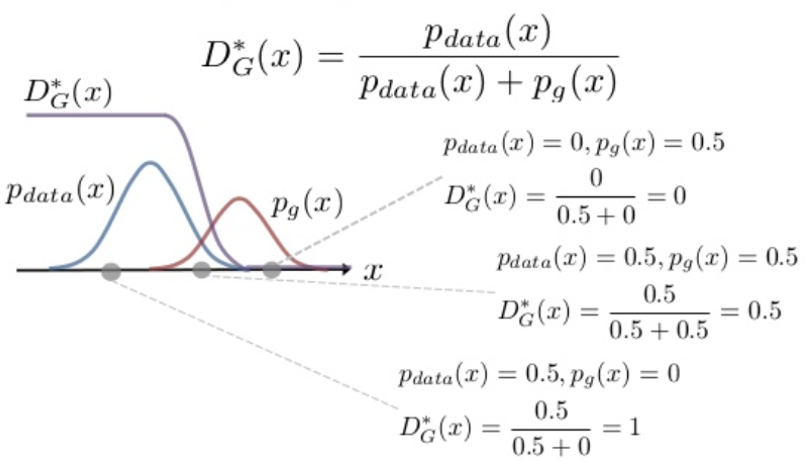
\includegraphics[width=7cm]{plots/opt_discriminator.png}}
      \tiny{\\Credit: Mark Chang}
  \end{figure}
   \begin{itemize}
  \item  The optimal discriminator returns a value greater than 0.5 if the probability to come from the data ($p_{data}(x)$)  is larger than the probability to come from the generator ($p_g(x)$).
  \end{itemize}
\end{frame}

\begin{frame} {Optimal Discriminator}

  For G fixed, the optimal discriminator $D^*_G$ is:
  \begin{figure}
    \centering
      \scalebox{1}{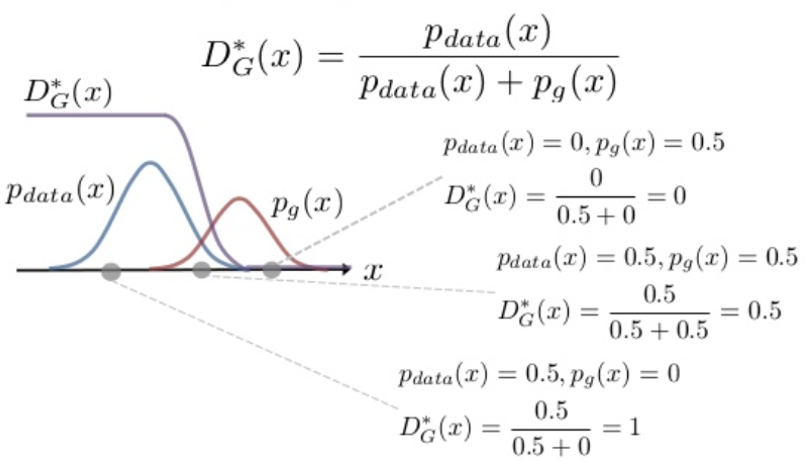
\includegraphics[width=7cm]{plots/opt_discriminator.png}}
      \tiny{\\Credit: Mark Chang}
  \end{figure}
  \begin{itemize}
  \item  Note: The optimal solution is almost never found in practice, since the discriminator has a finite capacity and is trained on a finite amount of data.
  \item Therefore, the assumption needed to guarantee that the generator minimizes the JSD does usually not hold in practice.
  \end{itemize}
\end{frame}

%

%--------------------------------------------
%
%---------------------------------------------
\section{Challenges for GAN Optimization}



\begin{frame} {Adversarial Training}  
  \vspace{2mm}
Deep Learning models (in general) involve a single player!
  \vspace{1mm}
  \begin{itemize}
    \item The player tries to maximize its reward (minimize its loss),
    \item Use SGD (with backprob) to find the optimal parameters,
    \item SGD has convergence guarantees (under certain conditions).
    \item However, with non-convexity, we might convert to local minima!
  \end{itemize}
    \vspace{3mm} 
GAN instead involve two players
     \vspace{1mm}
  \begin{itemize}
    \item Discriminator is trying to maximize its reward,
    \item Generator is trying to minimize discriminator's reward.
    \item  SGD was not designed to find the Nash equilibrium of a game!
    \item Therefore, we might not converge to the Nash equilibrium at all!
  \end{itemize}
%   \vspace{3mm}
%(*) SGD was not designed to find the Nash equilibrium of a game! \\
  \vspace{2mm}
%(**) Therefore, we might not converge to the Nash equilibrium at all!
      
 \end{frame}
 
% \begin{frame} {Adversarial Training - Example}
 
%     \begin{itemize}
%      \item Assume, we have two players A and B:
%      \begin{itemize}
%      \item $ \min \limits_x \max \limits_y V (x,y)$
%      \item This can be rewritten as $V(x,y) = xy$.
%      \end{itemize}
%     \end{itemize}
% 
%    \begin{figure}
%    \centering
%      {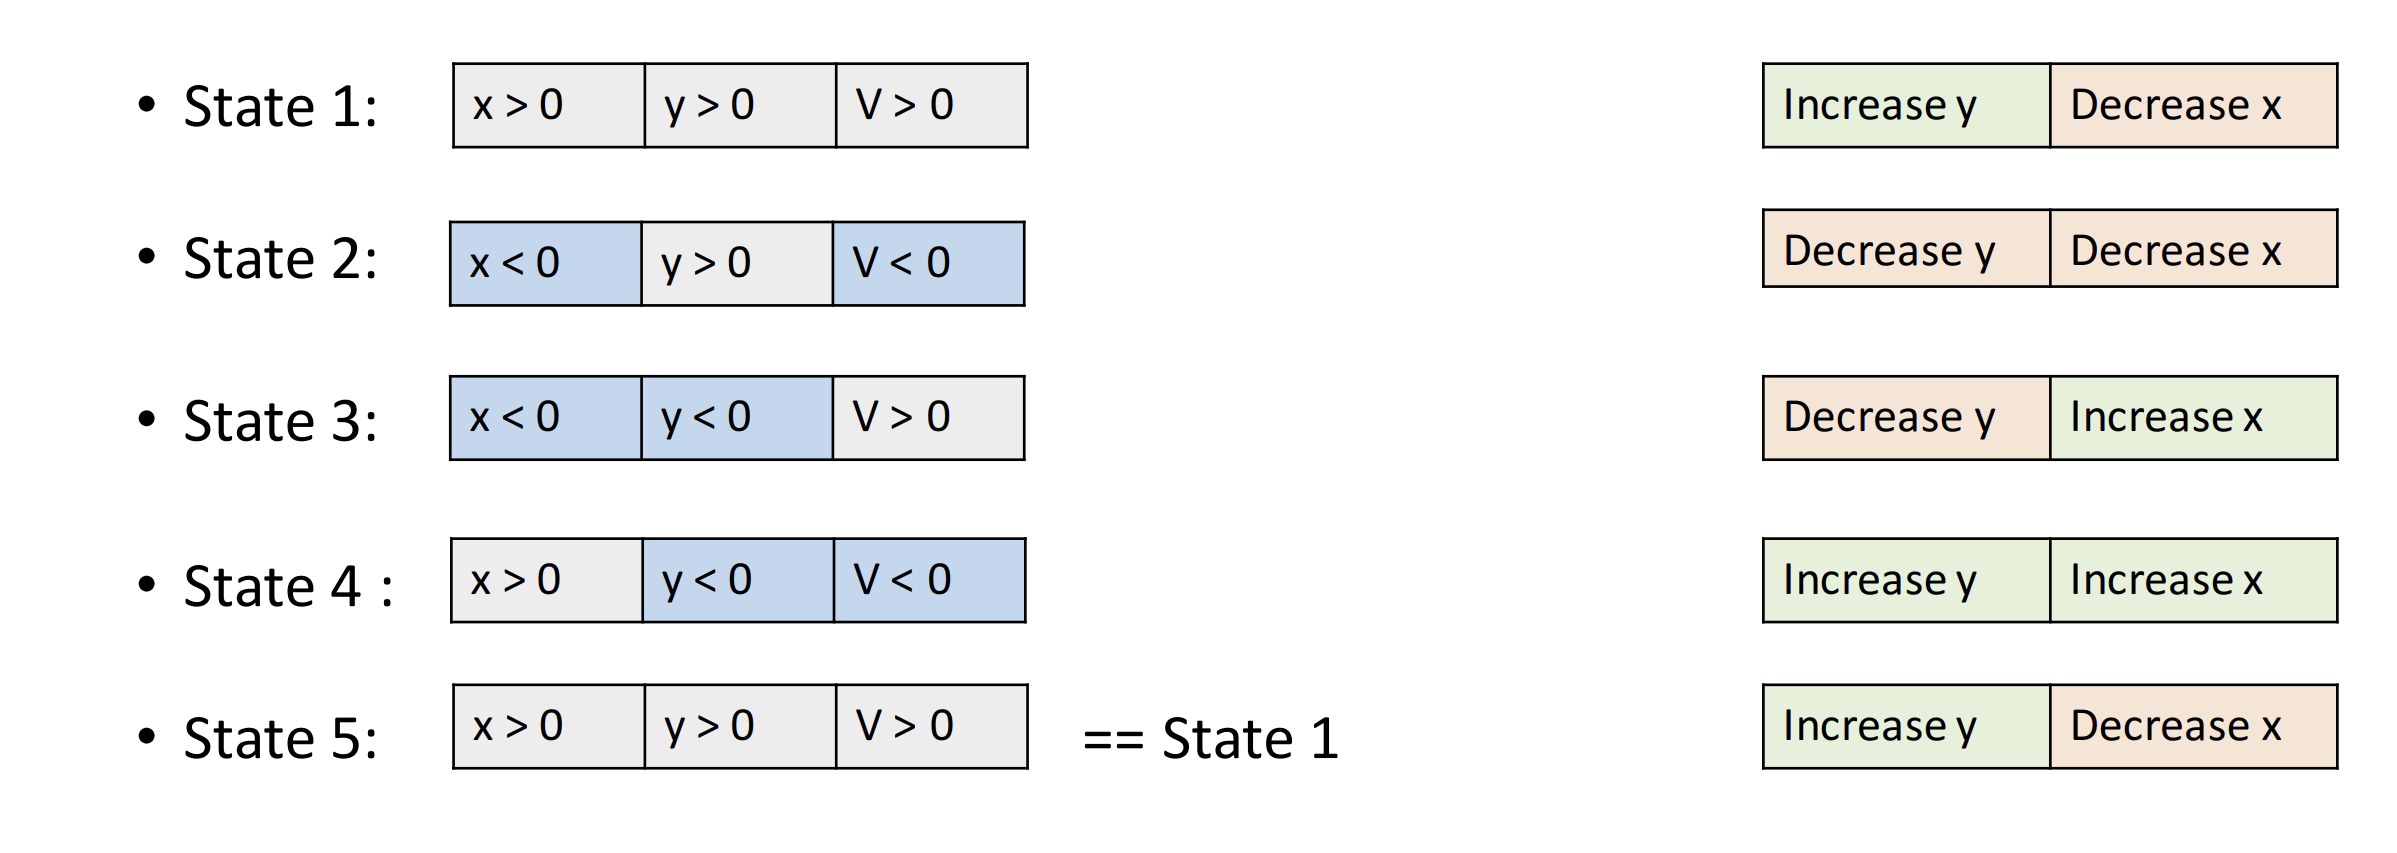
\includegraphics{plots/nonconverge.png}}
      %\tiny{\\Credit: https://slazebni.cs.illinois.edu/spring17/lec11_gan.pdf}
%   \end{figure}

%\end{frame}

%-------------------
%\begin{frame} {Adversarial Training}
%\begin{itemize}
%\vspace{12mm}
%\item So, GANs have intuitive appeal and produce state-of-the-art results but the reason they are such an important breakthrough is that they introduce a whole new paradigm to training deep neural networks: Adversarial Training$^1$.
%\vspace{4mm}
%\item Compared to plain-vanilla gradient descent, 
%adversarial training is a whole different beast; one that we have not figured out how to tame (yet).
%\vspace{4mm}
%\item To illustrate this, let us look at a simple example.
%\vspace{6mm}
%\end{itemize}
%\tiny{1. The term 'adversarial training' is used in slightly different contexts in the community. }
%\end{frame}

\begin{frame} {Adversarial Training -Example}
\begin{figure}
\centering
\scalebox{0.9}{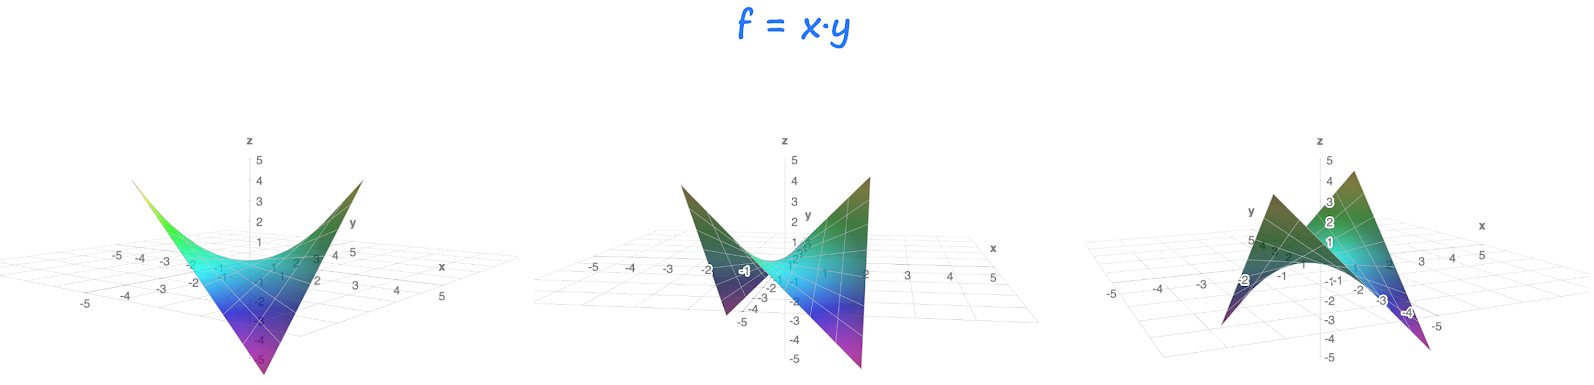
\includegraphics{plots/adv_xy.png}}
\end{figure}
\begin{itemize}
\item Consider the function $f(x,y) = xy$, where $x$ and $y$ are both scalars.
\item Player A can control $x$ and Player B can control $y$.
    \item The loss:
    \begin{itemize}
\item Player A: $L_{A}(x,y) = xy$
    \item Player B: $L_{B}(x,y) = -xy$
    \end{itemize}
\item This can be rewritten as $L(x,y) = \min \limits_x \max \limits_y xy$
    \item What we have here is a simple zero-sum game with its characteristic minimax loss.
\end{itemize}
\end{frame}

    
\begin{frame} {Possible behaviour \#1: Convergence}
  \begin{figure}
    \centering
     {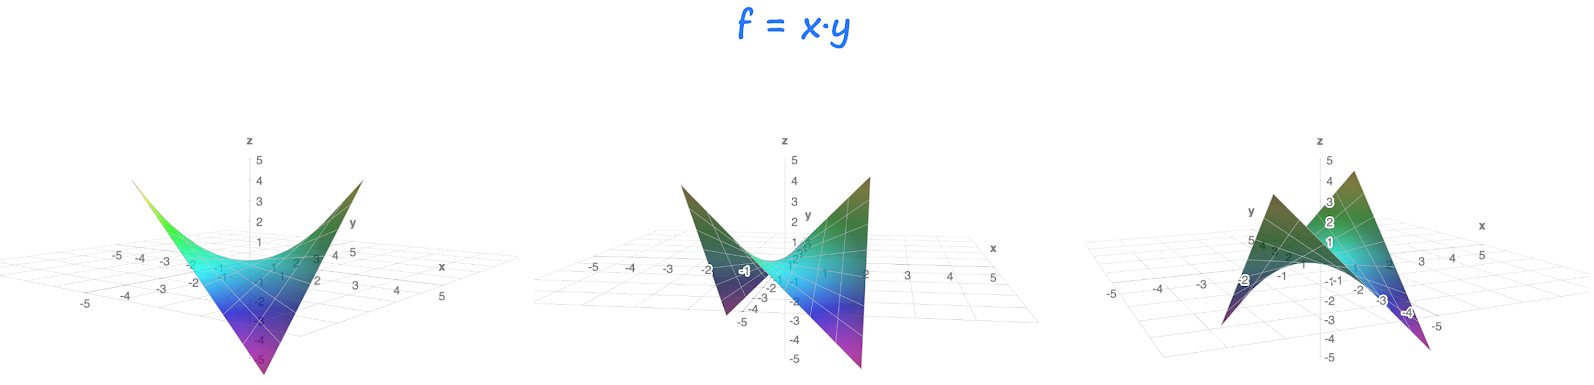
\includegraphics{plots/adv_xy.png}}
  \end{figure}
  \begin{itemize}
    \item The partial derivatives of the losses are:
     \begin{equation*}
       \frac {\partial{L_{A}}}{\partial x} = y \text{ , }
       \frac {\partial{L_{B}}}{\partial y} = -x
     \end{equation*}
    \item In adversarial training, both players perform gradient descent on their respective losses.
    \item %To perform simultaneous gradient descent, 
    We update $x$ with $x - \alpha \cdot y$ and $y$ with $y + \alpha \cdot x$ simultaneously in one iteration, where $\alpha$ is the learning rate.
  \end{itemize}
\end{frame}

\begin{frame} {Possible behaviour \#1: Convergence}
  \begin{figure}
    \centering
      \scalebox{0.9}{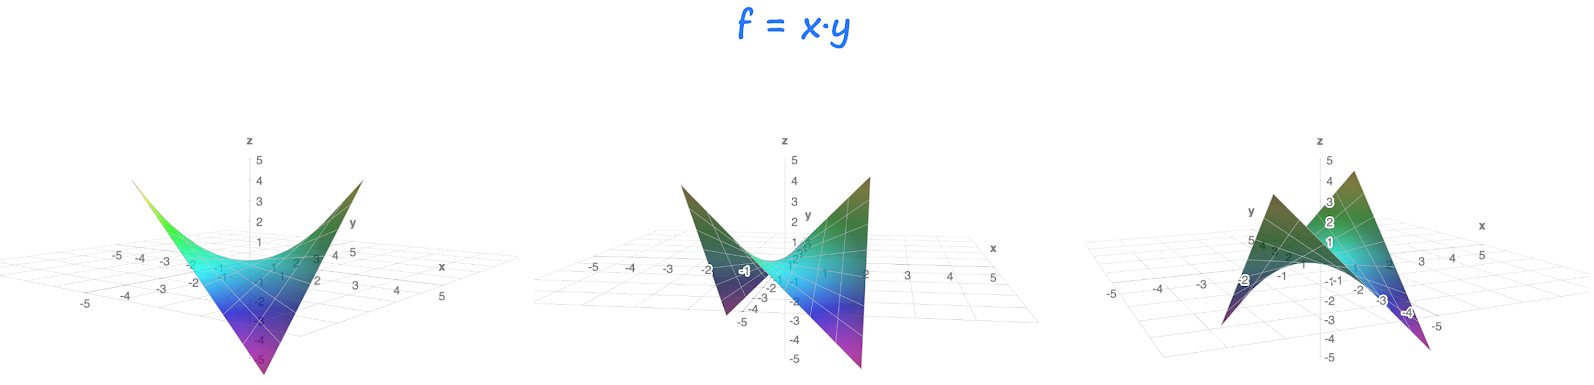
\includegraphics{plots/adv_xy.png}}
  \end{figure}
  \begin{itemize}
    \item In order for simultaneous gradient descent to converge to a fixed point, both gradients have to be simultaneously 0.
    \item They are both (simultaneously) zero only for the point (0,0).
    \item This is a saddle point of the function $f(x,y) = xy$.
    \begin{itemize}
       \item The fixed point for a minimax game is typically a saddle point.
      \item Such a fixed point is an example of a Nash equilibrium.
    \end{itemize}
    \item In adversarial training, convergence to a fixed point is \textbf{not} guaranteed.
  \end{itemize}
\end{frame}

\begin{frame} {Possible behaviour \#2: Chaotic behaviour}
  \begin{figure}
    \centering
      \scalebox{0.6}{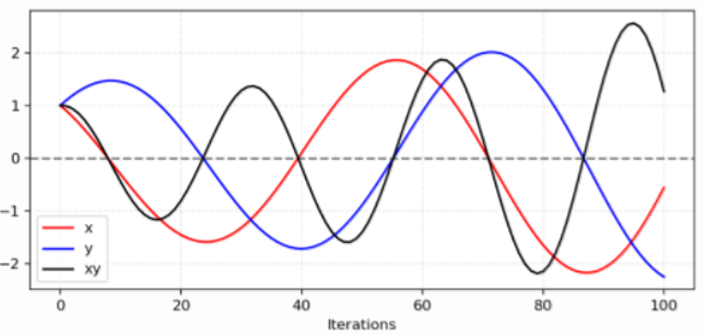
\includegraphics{plots/sim_grad.png}}
      \tiny{\\Credit: Lilian Weng}
      \caption{\footnotesize A simulation of our example for updating x to minimize xy and updating y to minimize -xy. The learning rate $\alpha$ = 0.1. With more iterations, the oscillation grows more and more unstable.}
  \end{figure}
  \begin{itemize}
    \item Once $x$ and $y$ have different signs, every following gradient update causes huge oscillation and the instability gets worse in time, as shown in the figure.
  \end{itemize}
\end{frame}


\begin{frame} {Possible behaviour \#3: Cycles}
  \begin{figure}
    \centering
      \scalebox{0.3}{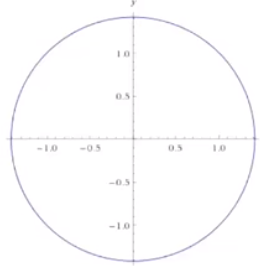
\includegraphics{plots/adv_cycle.png}}
      \tiny{\\Credit: Goodfellow}
      \caption{\footnotesize Simultaneous gradient descent with an infinitesimal step size can result in a circular orbit in the parameter space.}
  \end{figure}
  \begin{itemize}
    \item A discrete example: A never-ending game of Rock-Paper-Scissors where player A chooses 'Rock' $\rightarrow$ player B chooses 'Paper' $\rightarrow$ A chooses 'Scissors' $\rightarrow$ B chooses 'Rock' $\rightarrow$ ...
   % \item In GAN training, this happens when the generator keeps switching the category of the samples generated without a noticeable improvement in image quality for any category.
   \item  \textbf{Takeaway:} Adversarial training is highly unpredictable. It can get stuck in cycles or become chaotic.
  \end{itemize}
\end{frame}


\begin{frame} {Non-stationary loss surface}
   \begin{itemize}
     \item %Once again, it is extremely important to note that 
     From the perspective of one of the players, the loss surface changes every time the other player makes a move.
  \vspace{2mm}
     \item This is in stark contrast to  (full batch) gradient descent where the loss surface is stationary no matter how many iterations of gradient descent are performed.
%  \vspace{2mm}
   %  \item It's \textit{somewhat} analogous to a game of football played by two players where the goalposts for a given player changes position every time the opponent kicks the ball and vice versa!
%   \vspace{2mm}
 %   \item The only way this game ends(\textit{if} it ends, that is) is if the ball goes through both players' goalposts simultaneously.
%   \vspace{2mm}
%    \item This is what a saddle point represents. It is simultaneously a minimum for the first player and a maximum for the second player.

   \end{itemize}
 \end{frame}

\begin{frame} {Illustration of Convergence}
  \begin{figure}
    \centering
      \scalebox{0.8}{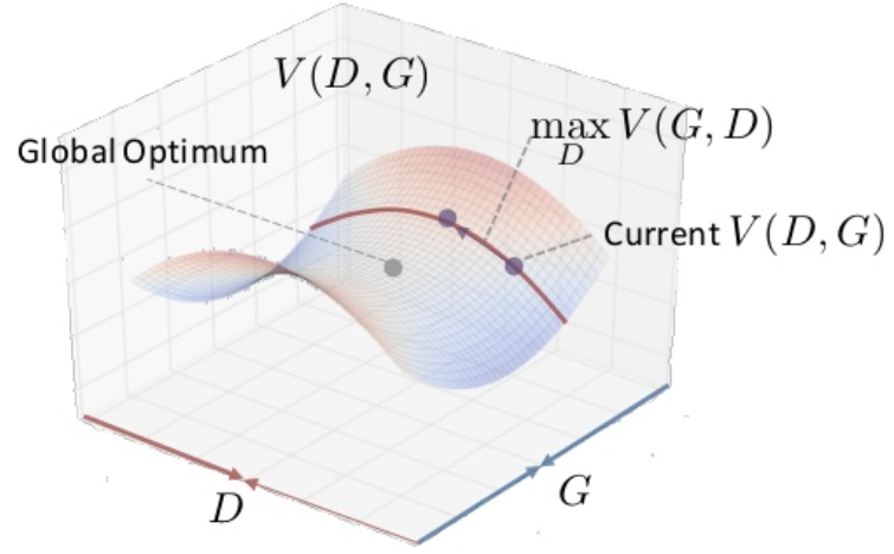
\includegraphics{plots/illus_conv_one.png}}
      \tiny{\\Credit: Mark Chang}
  \end{figure}
\end{frame}

\begin{frame} {Illustration of Convergence: Final Step}
  \begin{figure}
    \centering
      \scalebox{0.8}{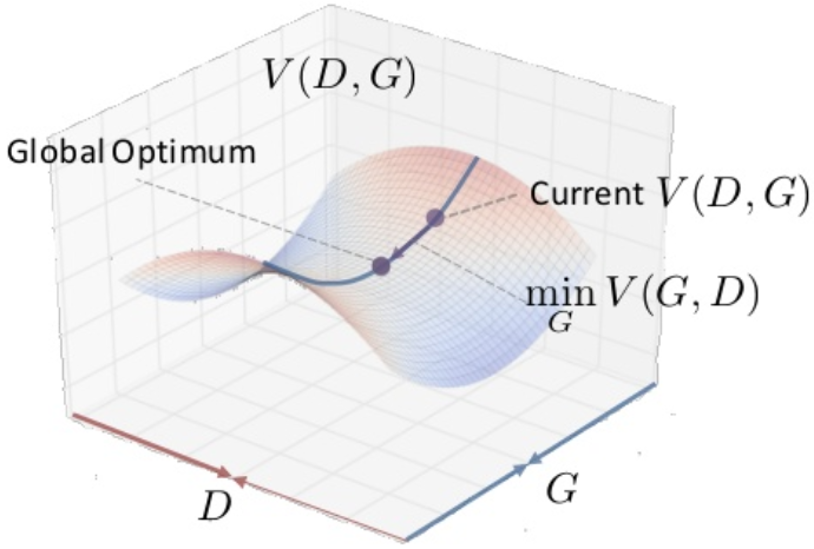
\includegraphics{plots/illus_conv_two.png}}
      \tiny{\\Credit: Mark Chang}
  \end{figure}
  Such convergence is not guaranteed, however.
\end{frame}

%\begin{frame} {Toy Example: Estimating a 1D Gaussian}
%  \vspace{10mm}
%  \begin{itemize}
%    \item Our target distribution is a simple Gaussian with mean 4 and standard deviation of 0.5.
%    \begin{figure}
%    \centering
%      \scalebox{0.66}{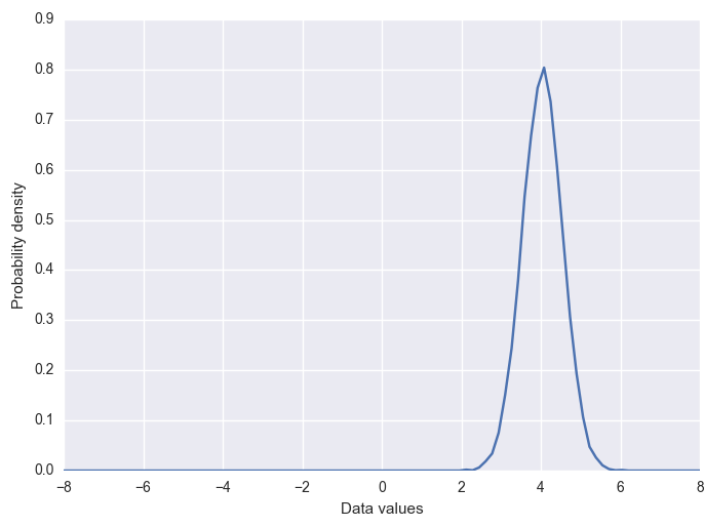
\includegraphics{plots/toy_gaussian.png}}
%      \tiny{\\Source: Aylien}
%  \end{figure}
%  \end{itemize}
%\end{frame}
%
%\begin{frame} {Toy Example: Estimating a 1D Gaussian}
%  \begin{itemize}
%    \item Our generator
%      \begin{itemize}
%        \item Takes a scalar noise input
%        \item Has only a single hidden layer with a softplus activation
%        \item The output layer has only a single neuron with a linear activation
%      \end{itemize}
%  \vspace{4mm}
%    \item Our discriminator
%      \begin{itemize}
%        \item Has 3 hidden layers with 'tanh' activations
%        \item The output layer once again has a single neuron with a sigmoid activation
%      \end{itemize}
%  \vspace{4mm}
%    \item Loss: Non-saturating Loss
%  \vspace{4mm}
%    \item Optimizer: Gradient Descent with exponential learning rate decay
%  \end{itemize}
%\end{frame}
%
%\begin{frame} {Toy Example: Estimating a 1D Gaussian}
%
%  \begin{itemize}
%  \item After training, the the two distributions look like this:
%  \begin{figure}
%    \centering
%      \scalebox{0.75}{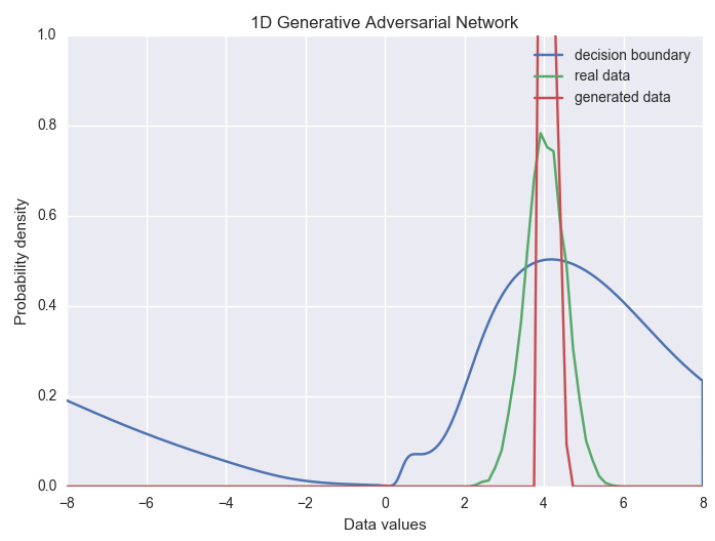
\includegraphics{plots/gan_gaussian_post.png}}
%      \tiny{\\Source: Aylien}
%  \end{figure}
%  \item This makes sense intuitively.If the generator just produces the mean value of the real data in this simple example, then it is going to be quite likely to fool the discriminator.
%  \end{itemize}
%\end{frame}

\begin{frame} {Challenges for GAN Training}

  \begin{itemize}
    \item Non-convergence: the model parameters oscillate, destabilize and never converge,
    \item Mode collapse: the generator collapses which produces limited varieties of samples,
     \item Diminished gradient: the discriminator gets too successful that the generator gradient vanishes and learns nothing,
     \item Unbalance between the generator and discriminator causing overfitting, 
     \item Highly sensitive to the hyperparameter selections.
  \end{itemize}
\end{frame}


%\begin{frame} {Mode collapse}
%\vspace{2mm}
%Real-life data distributions are multimodal. For example, in MNIST, there are 10 major modes from digit '0' to digit '9'. The samples below are generated by two different GANs. The top row produces all 10 modes while the second row creates a single mode only (the digit '6'). This problem is called mode collapse when only a few modes of data are generated. 
%\vspace{2mm}
%  \begin{figure}
%    \centering
%      \scalebox{1}{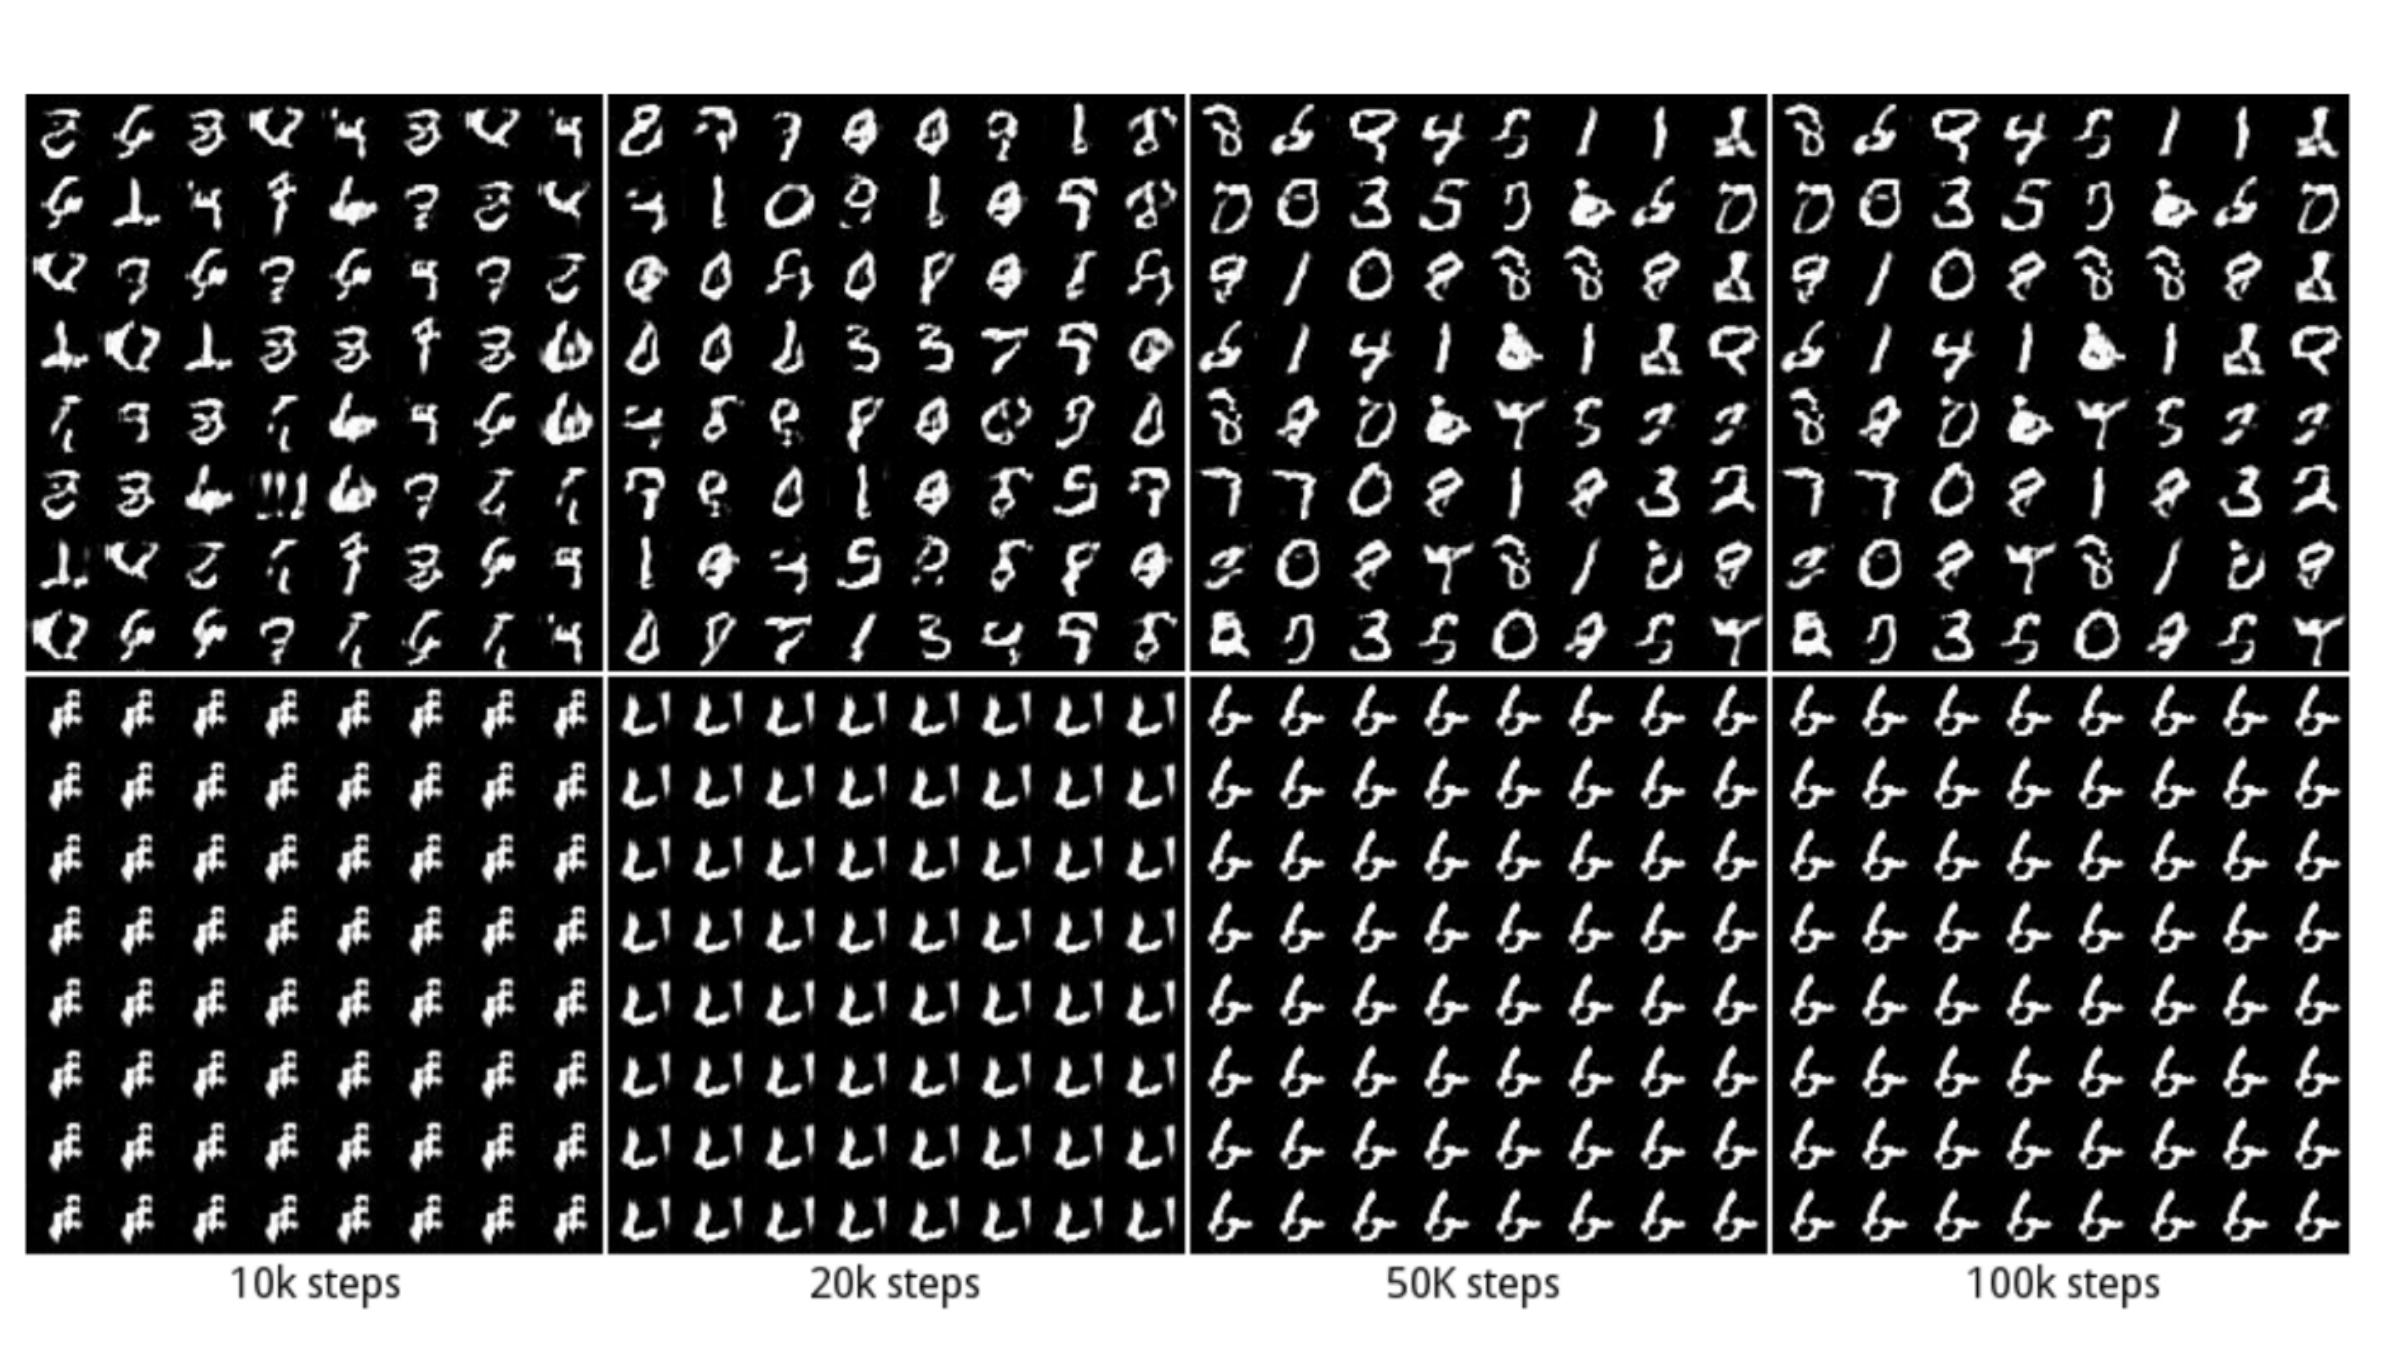
\includegraphics[width=7cm]{plots/modecollapse_mnist.png}}
%      \tiny{\\Credit: Luke Metz et al.(2017)}
%  \end{figure}
%\end{frame}

%\begin{frame} {Mode collapse- Example}
%\vspace{2mm}
%Generator fails to output diverse samples on Toy dataset
%\vspace{2mm}
%  \begin{figure}
%    \centering
%      \scalebox{1}{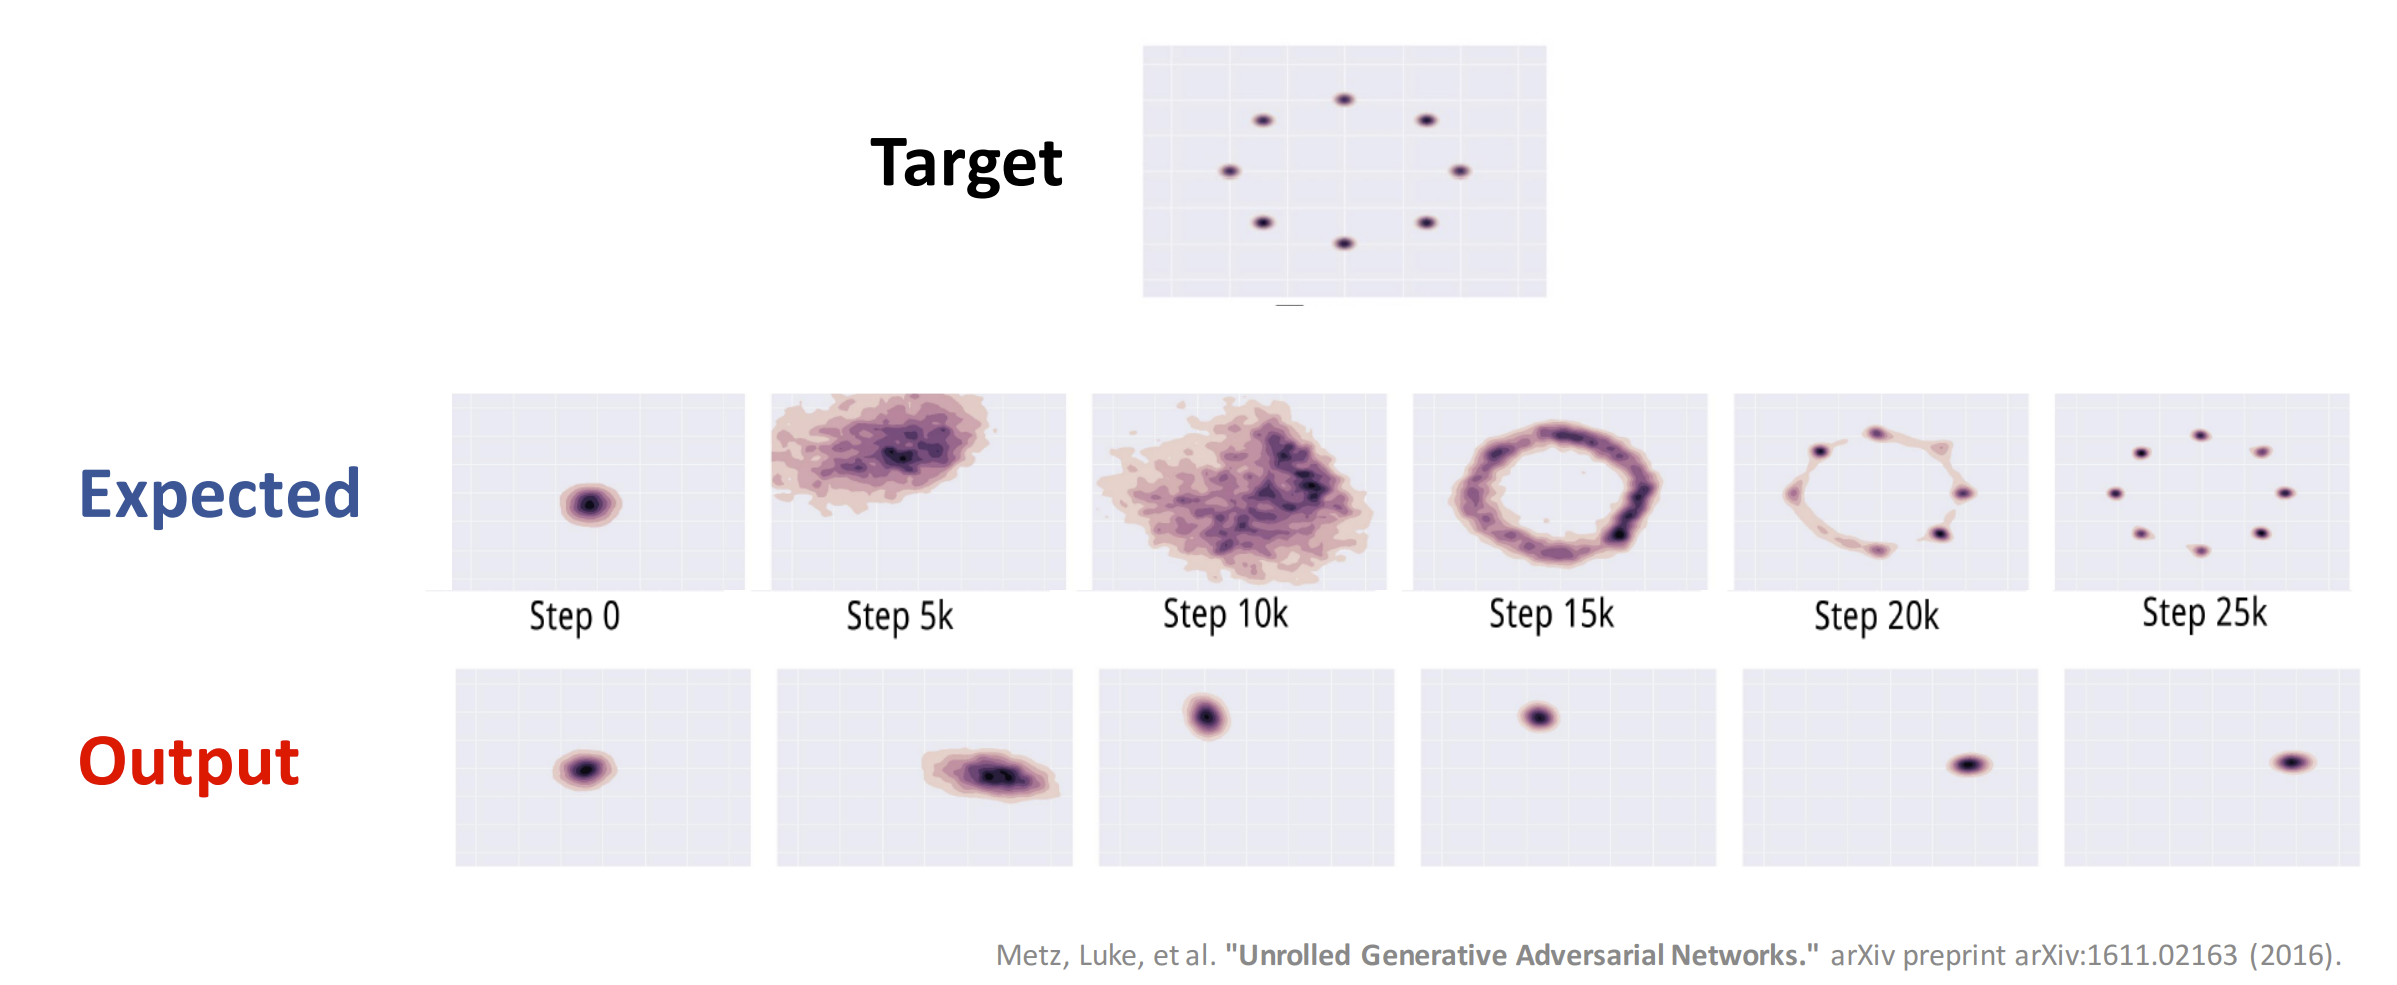
\includegraphics[width=12cm]{plots/toy.png}}
%  \end{figure}
%\end{frame}
%
%
%\begin{frame} {Solutions to tackle Mode Collapse}
%\vspace{2mm}
%  \begin{itemize}
%    \item Mini-batch GAN:
%      \begin{itemize}
%        \item Problem: Generator produces good samples but a very few of them, therefore discriminator can not tag them as fake!
%        \item Solution: Let the discriminator look at the entire batch instead of single example, If there is lack of diversity mark them fake! 
%        \item Result: Generator will be force to produce diverse samples!
%      \end{itemize}
%    \item Train with labels
%          \begin{itemize}
%            \item Label information of real data might help
%            \item Here, we train D with all categories instead of binary label!
%          \end{itemize}
%  \end{itemize}
%\end{frame}

%\begin{frame} {Vanishing gradients in JS-Divergence}
%\vspace{2mm}
%  \begin{itemize}
%    \item Recall that when the discriminator is optimal, the objective function for the generator is:\\
%     $\min \limits_G V(D^*,G) = 2 D_{JS} (p_r || p_g) - 2 \log 2 $
%    \vspace{2mm}
%    \item  The problem happens when the data distribution $q$ of the generator's images does not match with the ground truth $p$ for the real images.
%    \item  Let's consider q with different means to study the gradient of $JS(p, q)$
%  \end{itemize}
%  
%    \begin{figure}
%    \centering
%      \scalebox{1}{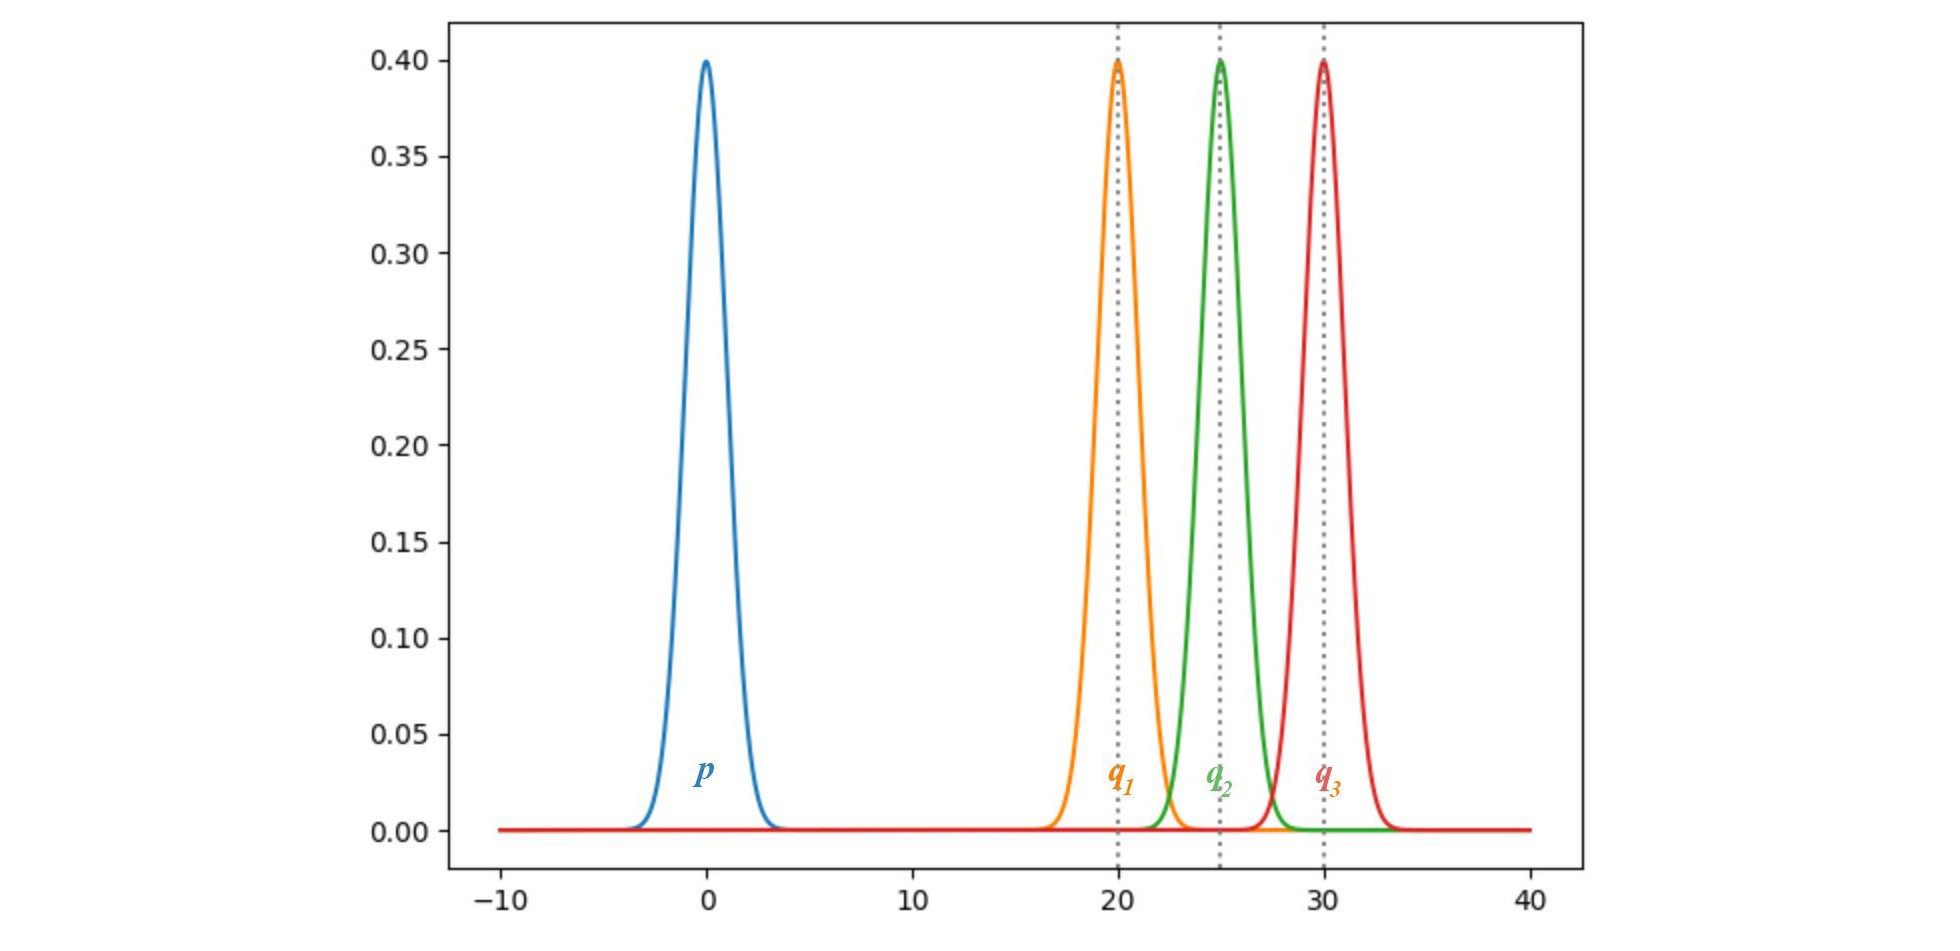
\includegraphics[width=7cm]{plots/JS1.jpeg}}
%      \tiny{\\Credit: Jonathan Hui.(2017)}
%  \end{figure}
%
%\end{frame}

%\begin{frame} {Vanishing gradients in JS-Divergence}
%    \vspace{2mm}
%    \begin{itemize}
%        \item Here, we plot the JS-divergence $JS(p, q)$ between $p$ and $q$ with means of $q$ ranging from 0 to 30. 
%\item As shown below, the gradient for the JS-divergence vanishes from $q_1$ to $q_3$.\\
%\item Results: The GAN generator will learn extremely slow to nothing when the cost is saturated in those regions. In early training, p and q are very different and the generator learns very slow.
%  \end{itemize}
%
%    \begin{figure}
%    \centering
%      \scalebox{1}{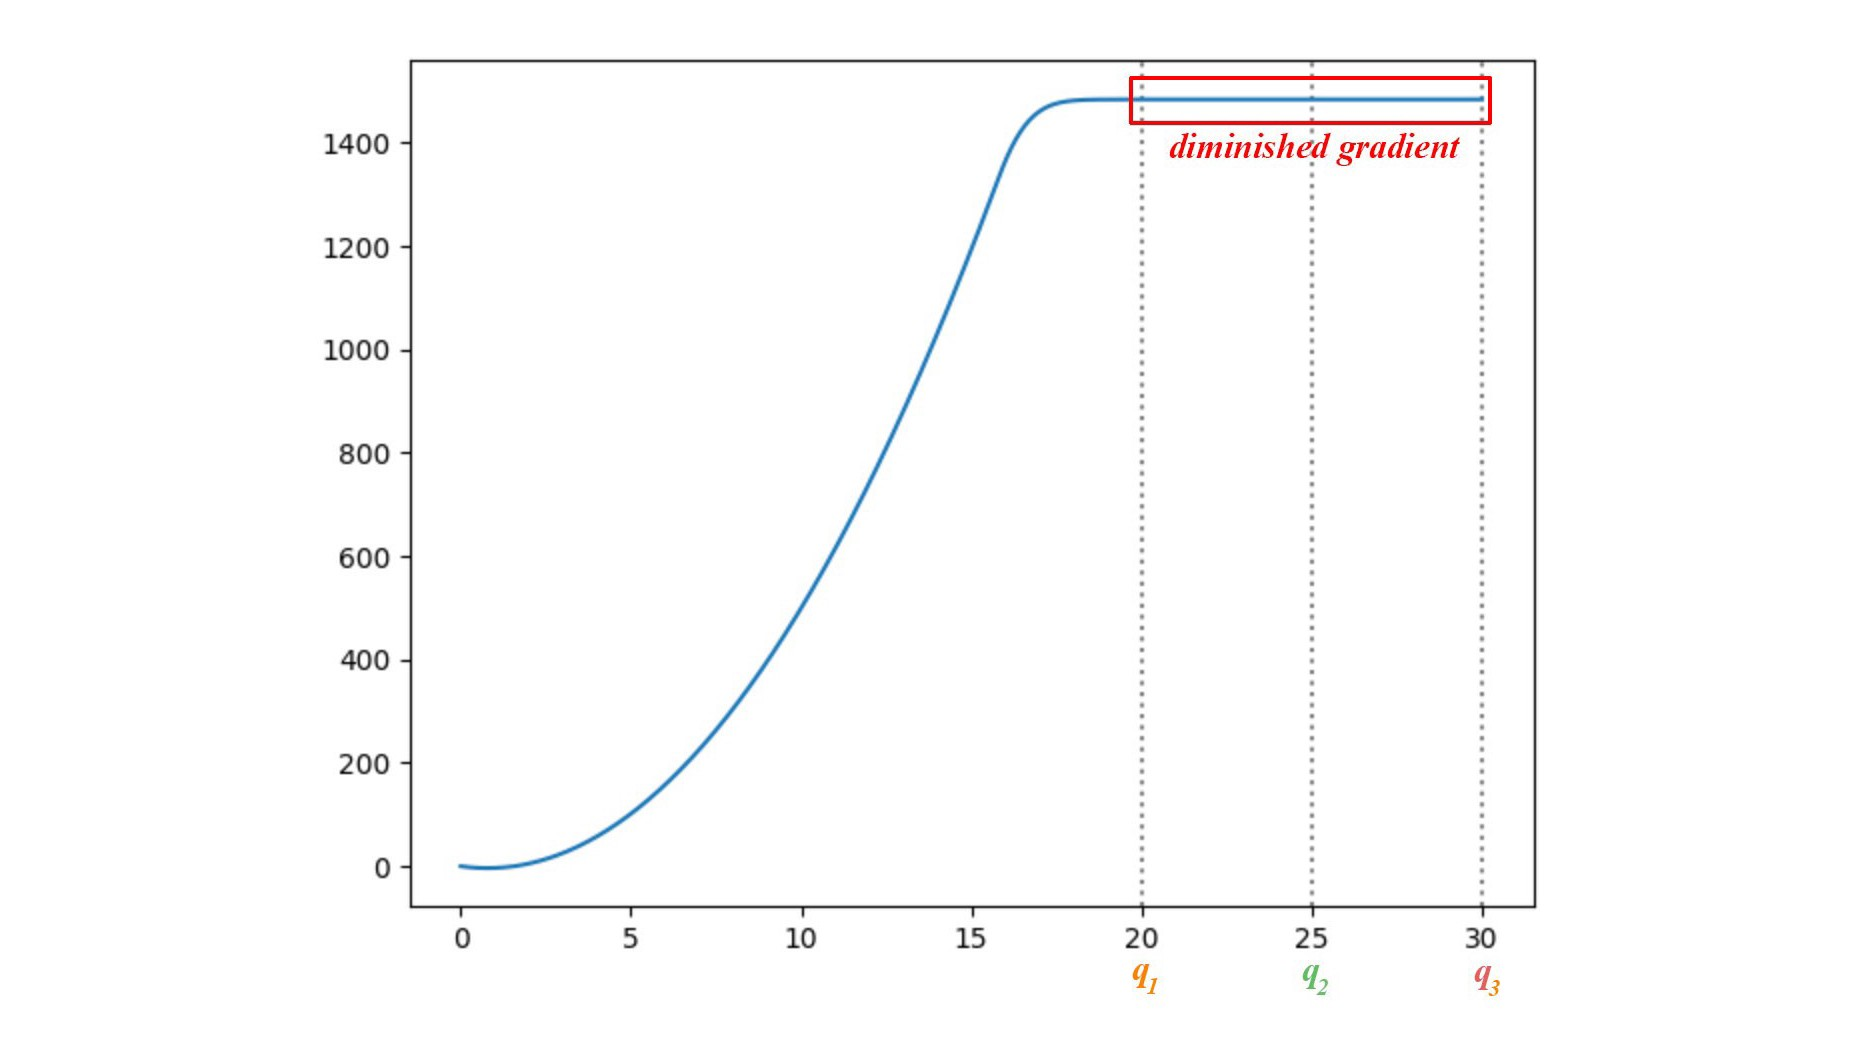
\includegraphics[width=7cm]{plots/JS2.jpeg}}
%      \tiny{\\Credit: Jonathan Hui.(2017)}
%  \end{figure}
%
%\end{frame}
%



%\begin{frame} {Trade-offs made by some common divergences}
%  \begin{figure}
%    \centering
%      \scalebox{1}{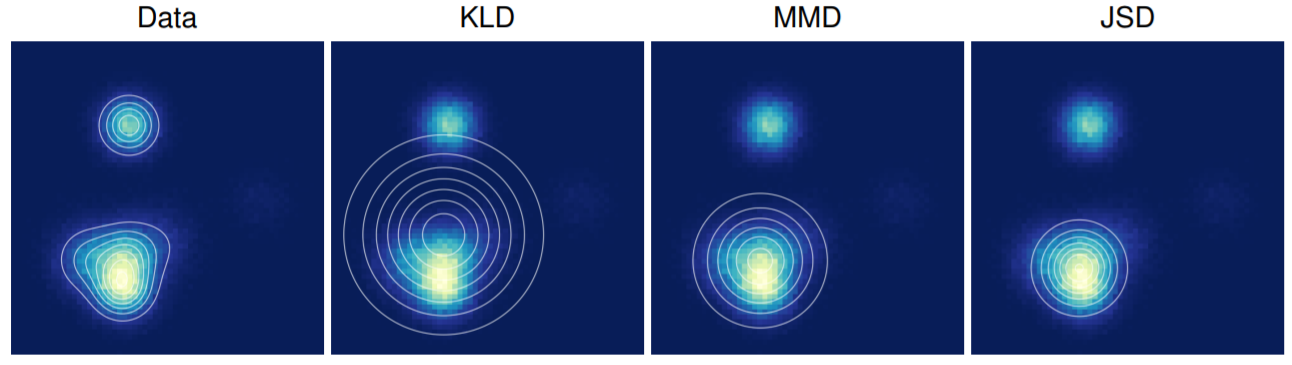
\includegraphics{plots/div_tradeoffs.png}}
%      \tiny{\\Source: Theis et al. 2016}
%      \caption{\small: An isotropic Gaussian distribution was fit to data drawn from a mixture of Gaussians by either minimizing Kullback-Leibler divergence (KLD), maximum mean discrepancy (MMD), or Jensen-Shannon divergence (JSD). The different fits demonstrate different tradeoffs made by the three measures of distance between distributions.}
% \end{figure}
%\end{frame}


%\begin{frame} {Trade-offs made by some common divergences}
%
%  \begin{figure}
%    \centering
%      \scalebox{0.8}{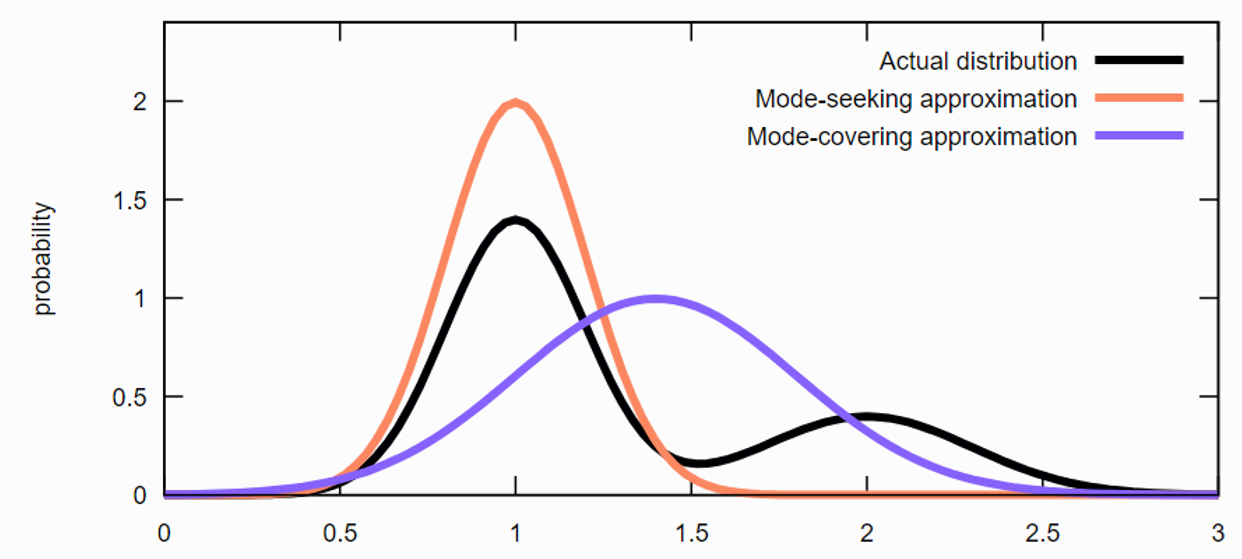
\includegraphics{plots/implicit_div.png}}
%      \tiny{\\Credit: Aiden NIbali}
%  \end{figure}
%  \begin{itemize}
%    \item In this simplified 1-dimensional example, $p_{\text{data}}(x)$ is a bimodal distribution, but $p_{\theta}(x)$ only has the modelling capacity of a single Gaussian.
%    \vspace{2mm}
%    \item Therefore, based on the divergence measure, $p_{\theta}(x)$ can either fit a single mode really well, i.e.~be `mode-seeking' (e.g.~JSD), or attempt to cover both modes, i.e. be `mode-covering' (e.g.~KLD).
%  \end{itemize}
%\end{frame}
%
%
%\begin{frame} {Alternative Divergences}
%
%Many common divergences, such as KL-divergence, Hellinger distance, and total variation distance, are special cases of f-divergence, coinciding with a particular choice of f. The following table lists many of the common divergences between probability distributions and the f function.
%
%  \begin{figure}
%    \centering
%      \scalebox{0.9}{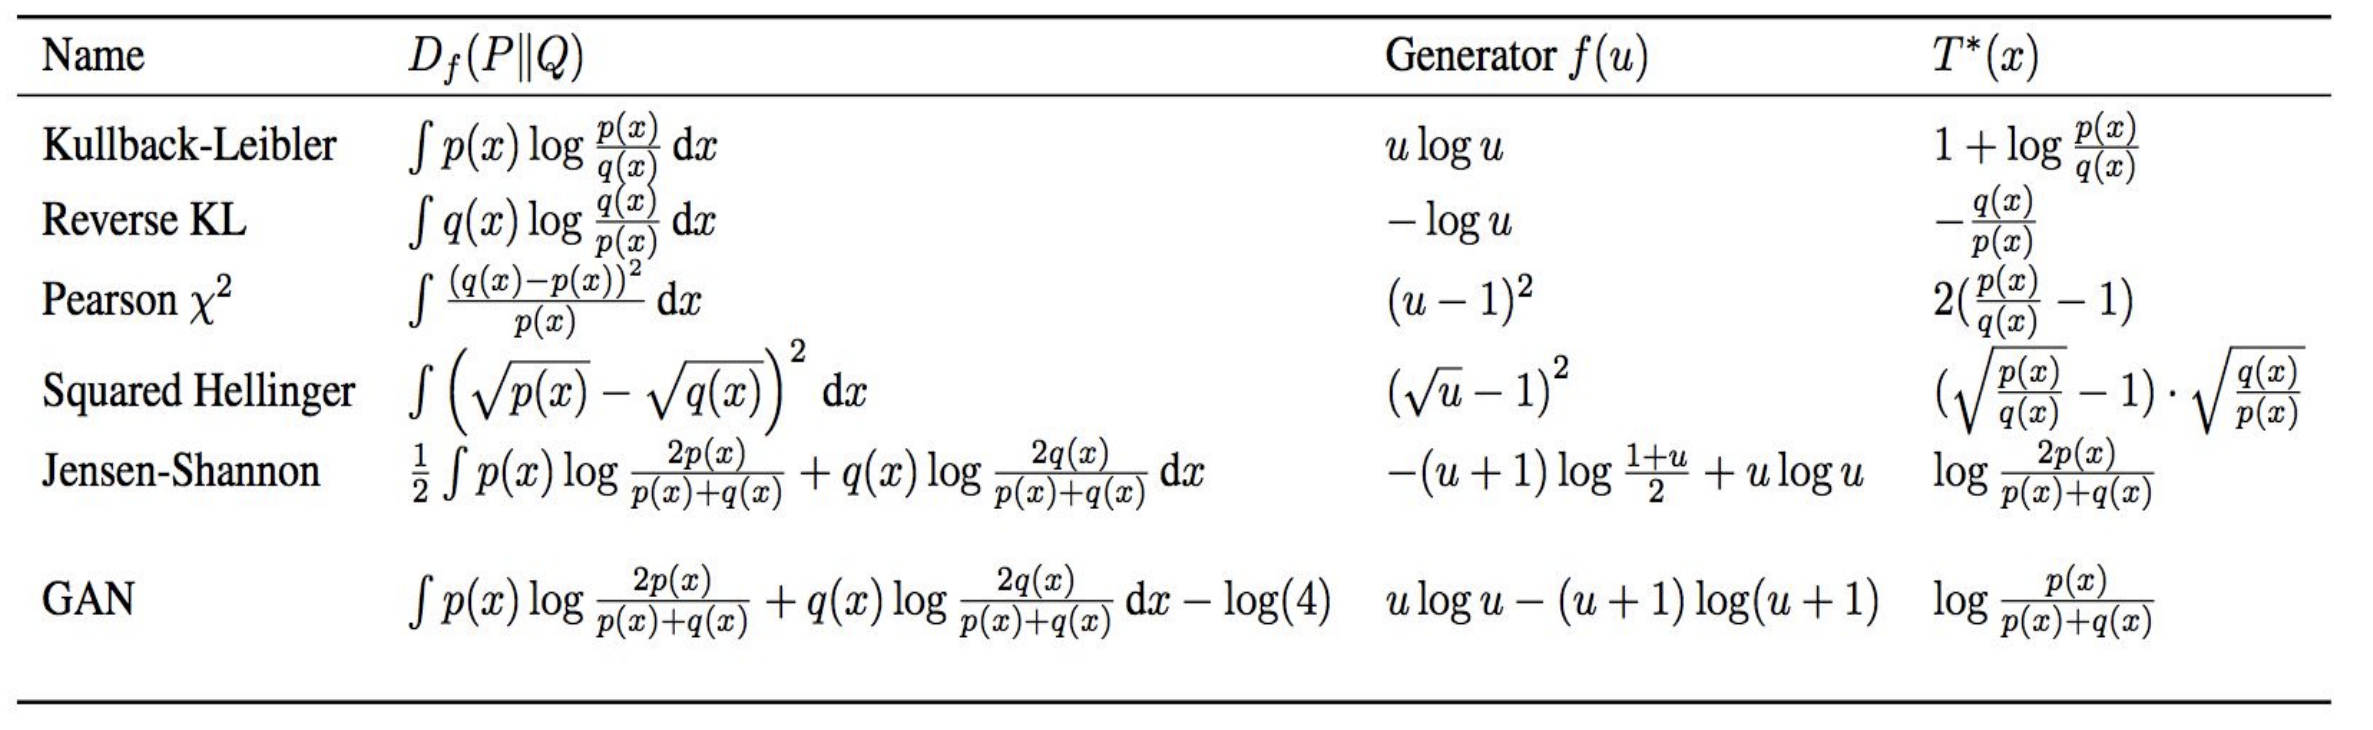
\includegraphics{plots/alternative_div.png}}
%      \tiny{\\Credit: Aiden NIbali}
%  \end{figure}
%  \begin{itemize}
%    \item We train a distribution $Q$ and an approximate the divergence with $T^{*}(x)$
%  \end{itemize}
%\end{frame}

%%%%-------------------------------------
\section{GAN variants}

\begin{frame} {Non-Saturating Loss}
  \begin{figure}
    \centering
      \scalebox{0.82}{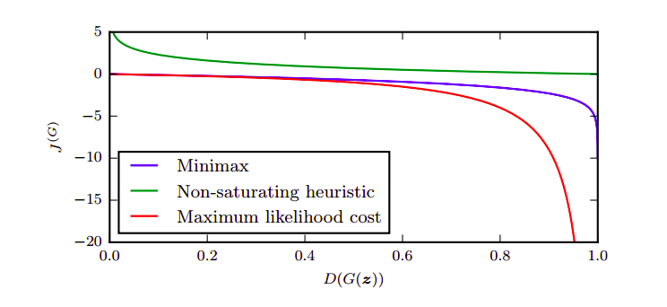
\includegraphics{plots/ns_loss.png}}
      \tiny{\\Credit: Daniel Seita}
      \caption{\footnotesize Various generator loss functions ($J^{(G)}$).}
  \end{figure}
  \begin{itemize}
    \item It was discovered that a relatively strong discriminator could completely dominate the generator.
    \item %The reason for this is that
   When optimizing the minimax loss, as the discriminator gets good at identifying fake images, i.e.~as $D(G(\mathbf{z}))$ approaches 0, the gradient with respect to the generator parameters vanishes.

  \end{itemize}
\end{frame}

\begin{frame} {Non-Saturating Loss}
  \begin{figure}
    \centering
      \scalebox{0.82}{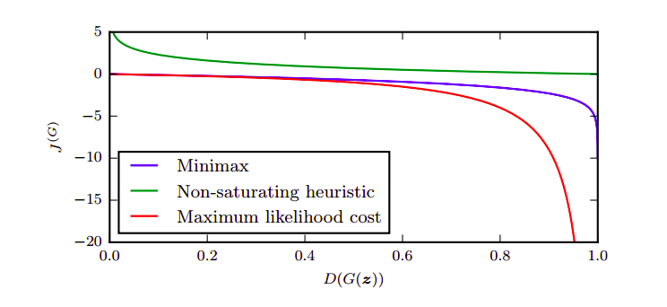
\includegraphics{plots/ns_loss.png}}
      \tiny{\\Credit: Daniel Seita}
      \caption{\footnotesize Various generator loss functions ($J^{(G)}$).}
  \end{figure}
  \begin{itemize}
    \item Solution: Use a non-saturating generator loss instead:  $J^{(G)} = - \frac{1}{2} \E_{\vec z \sim p(\vec z)} [\log D(G(\mathbf{x}))]$
    \item In contrast to the minimax loss, when the discriminator gets good at identifying fake images, the magnitude of the gradient of $J^{(G)}$ increases and the generator is able to learn to produce better images in successive iterations.
  \end{itemize}
\end{frame}


\begin{frame} {Other loss functions}

Various losses for GAN training with different properties have been proposed:

  \vspace{10mm}
  \begin{figure}
    \centering
      \scalebox{1}{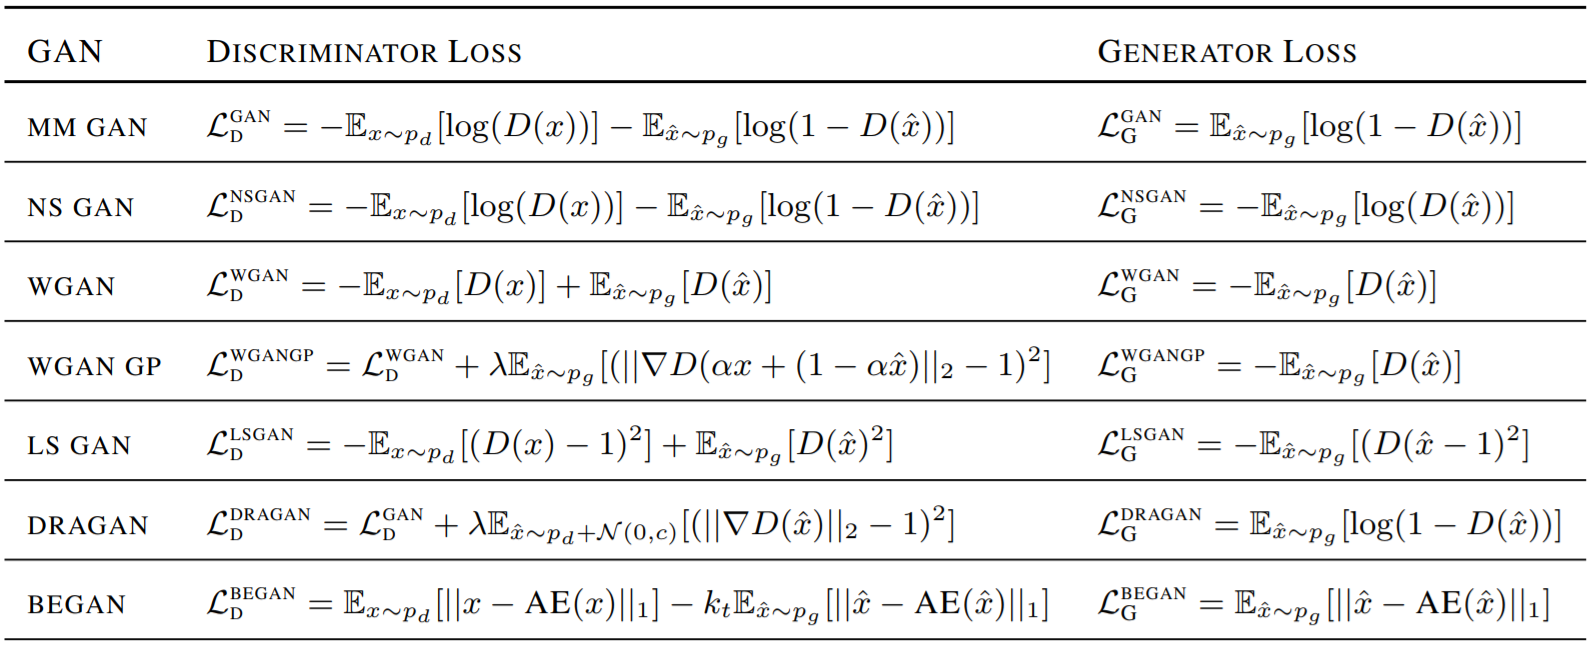
\includegraphics{plots/other_losses.png}}
      \tiny{\\Source: Lucic et al. 2016}
  \end{figure}
\end{frame}


%-------------------------------------
%\section{Architecture-variant GANs}

\begin{frame} {Architecture-variant GANs}

\vspace{2mm}
Motivated by different challenges in GAN training procedure described, there have been several types of architecture variants proposed.
\vspace{2mm}
Understanding and improving GAN training is a very active area of research.

  \begin{figure}
    \centering
      \scalebox{0.8}{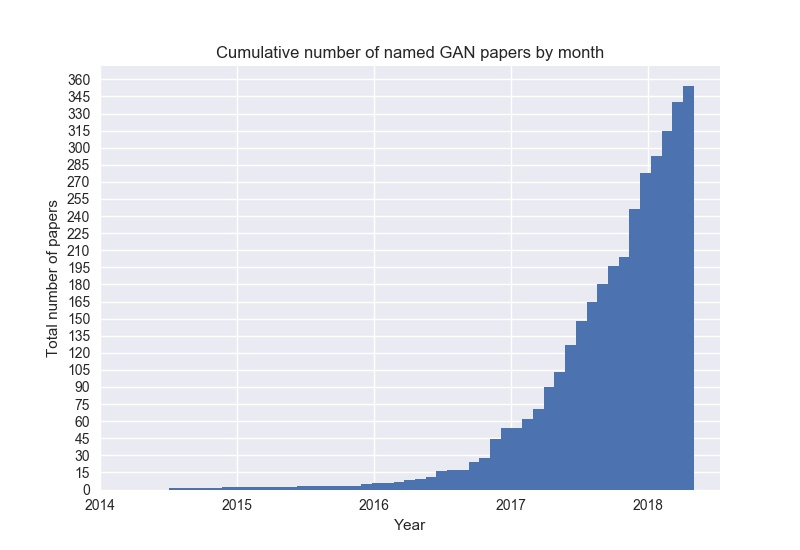
\includegraphics{plots/named_gans.png}}
      \tiny{\\Credit: hindupuravinash}
  \end{figure}
  \end{frame}
 
 \begin{frame} {GAN Application}
 
 What kinds of problems can GANs address?
  \begin{itemize}
    \item Generation
    \item Conditional Generation
    \item Clustering
    \item Semi-supervised Learning
    \item Representation Learning
    \item Translation
    \item Any traditional discriminative task can be approached with
generative models
  \end{itemize}

\end{frame}



\begin{frame} {Conditional GANs: Motivation}
  \begin{itemize}
    \item In an ordinary GAN, the only thing that is fed to the generator are the latent variables $\mathbf{z}$.
    \item A conditional GAN allows you to condition the generative model on additional variables. %have more control over the samples produced by the generator. This makes it very easy to work with multiple modalities.
    \item E.g. a generator conditioned on text input (in addition to $\mathbf{z}$) can be trained to generate the image described by the text.
  \end{itemize}
\end{frame}

\begin{frame} {Conditional GANs: Architecture}
  \begin{figure}
    \centering
      \scalebox{0.75}{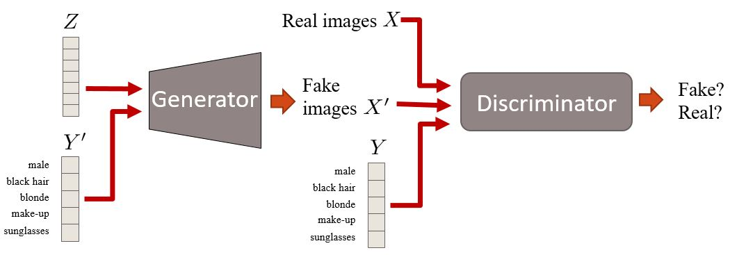
\includegraphics{plots/cgan_arch.png}}
      \tiny{\\Credit: Guim Perarnau}
  \end{figure}
  \begin{itemize}
    \item In a conditional GAN, additional information in the form of vector $\vec y$  is fed to both the generator and the discriminator.
    \item $\vec z$  can then encode all  variations in $\vec z$ that are not encoded by $\vec y$.
    \item E.g.~ $\vec y$ could encode the class of a hand-written number (from 0 to 9). Then,  $\vec z$ could encode  the style of the number (size, weight, rotation, etc).
  \end{itemize}
\end{frame}

%\begin{frame} {Conditional GANs: Loss}
%\end{frame}

\begin{frame} {Conditional GANs: Example}
  \vspace{10mm}
  \begin{figure}
    \centering
      \scalebox{1}{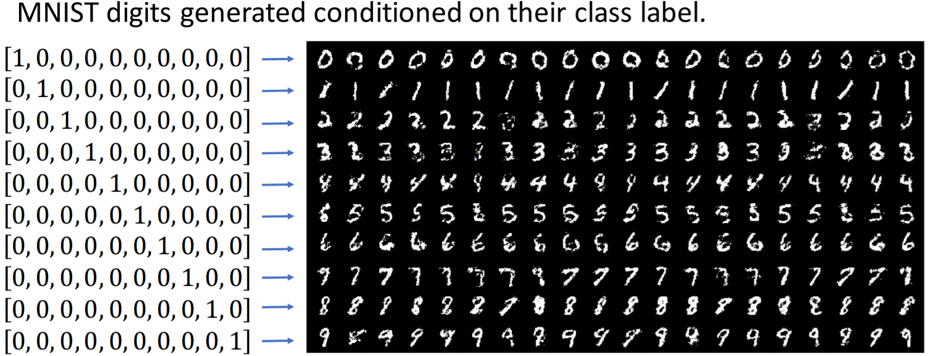
\includegraphics{plots/cgan_mnist.png}}
      \tiny{\\Source: Mirza et al. 2014}
      \caption{\footnotesize When the model is conditioned on a one-hot coded class label, it generates random images that belong (mostly) to that particular class. The randomness here comes from the randomly sampled $\mathbf{z}$. (Note : $\mathbf{z}$ is implicit. It is not shown above.)}
  \end{figure}
\end{frame}

\begin{frame} {Conditional GANs: More Examples}
  \begin{figure}
    \centering
      \scalebox{1}{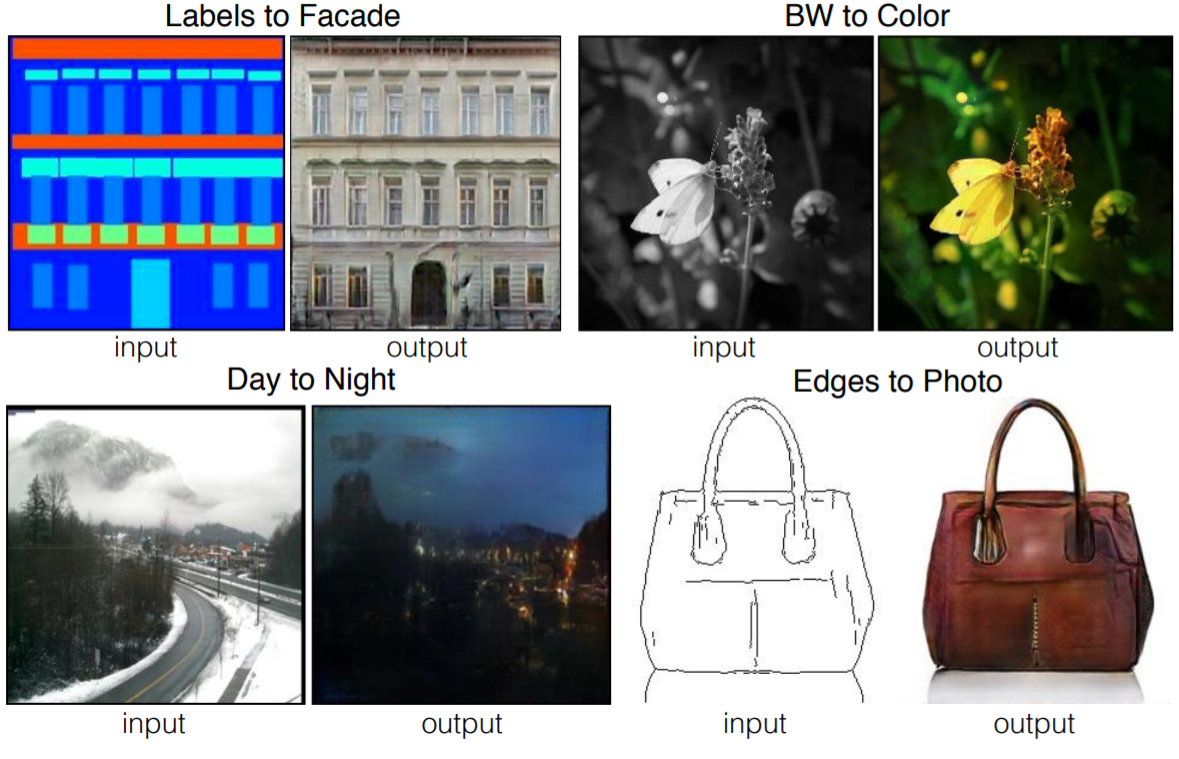
\includegraphics{plots/congan.png}}
       \tiny{\\Source: Isola et al. 2016}
       \caption{\footnotesize Conditional GANs can translate images of one type to another. In each of the 4 examples above, the image on the left is fed to the network and the image on the right is generated by the network.}
 \end{figure}
\end{frame}


\begin{frame} {More Generative Models}
  \begin{itemize}
   \vspace{8mm}
   \item Today, we learned about two kinds of (directed) generative models:
      \begin{itemize}
      \vspace{-0.4cm}
        \item Variational Autoencoders (VAEs)
        \item Generative Adversarial Networks (GANs).
      \end{itemize}
   \item There are other interesting generative models, e.g.:
      \begin{itemize}
        \item autoregressive models
        \item restricted Boltzmann machines.
      \end{itemize}
    \item Note:
      \begin{itemize}
        \item It is important to bear in mind that generative models are not a solved problem.
        \item There are many interesting hybrid models that combine two or more of these approaches.
      \end{itemize}
  \end{itemize}
\end{frame}

%\section{GAN Evaluation}

%\begin{frame} {GAN Evaluation}

%What makes a good generative model?
 % \begin{itemize}
%    \item Each generated sample is indistinguishable from a real sample
%    \item Generated samples should have variety
%  \end{itemize}
%  
%   \begin{figure}
%    \centering
%    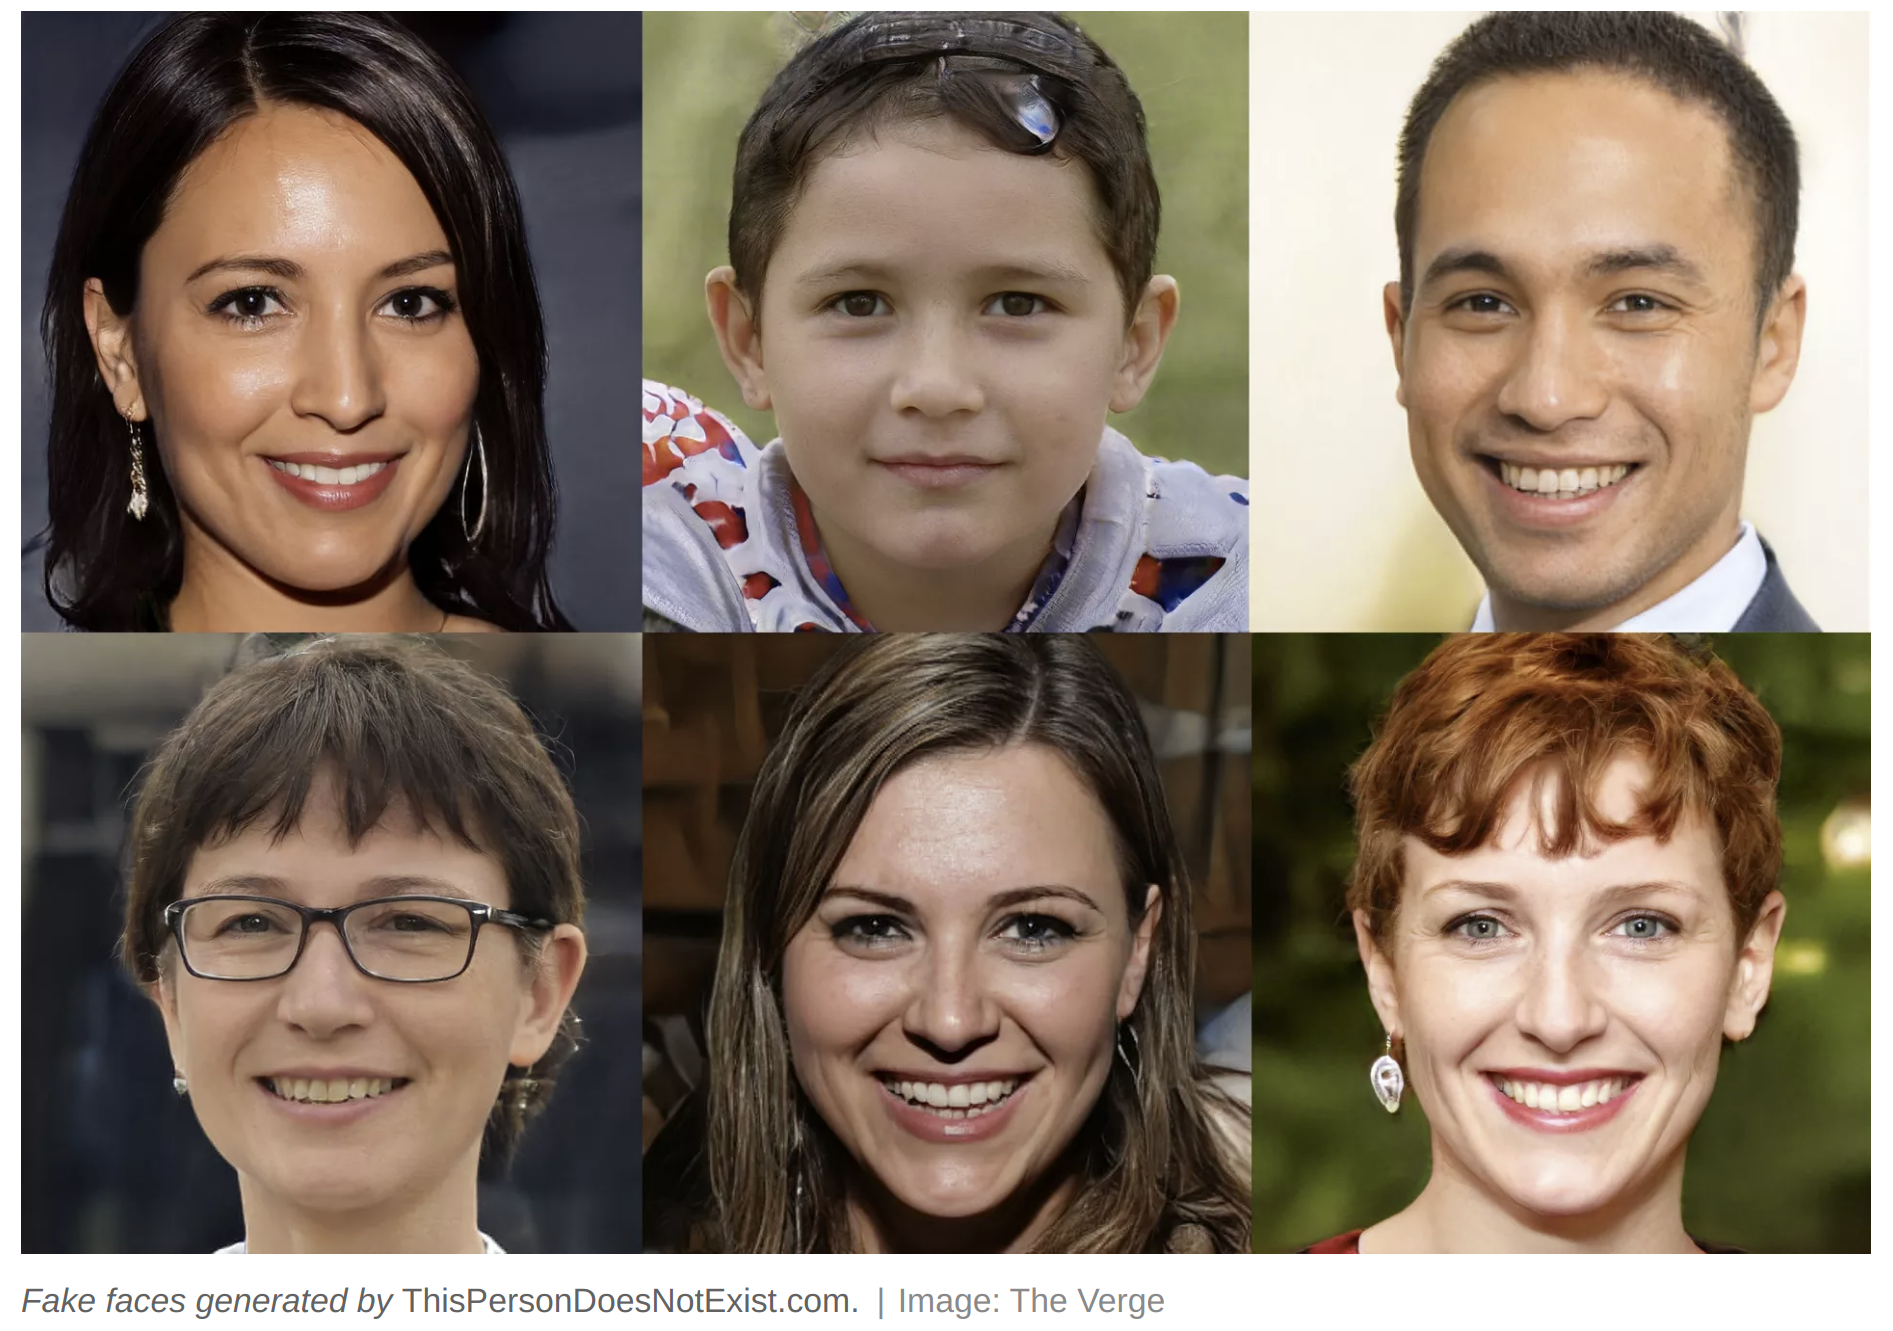
\includegraphics[width=8cm]{plots/exampleGAN.png}
%   \end{figure}
%\end{frame}
%
%
%\begin{frame} {GAN Evaluation}
%\vspace{2mm}
%How to evaluate the generated samples?
%
%  \begin{itemize}
% \item Cannot rely on the models' loss 
% \item Human evaluation
% \item Use a pre-trained model
%  \end{itemize}
%  
%   \begin{figure}
%    \centering
%    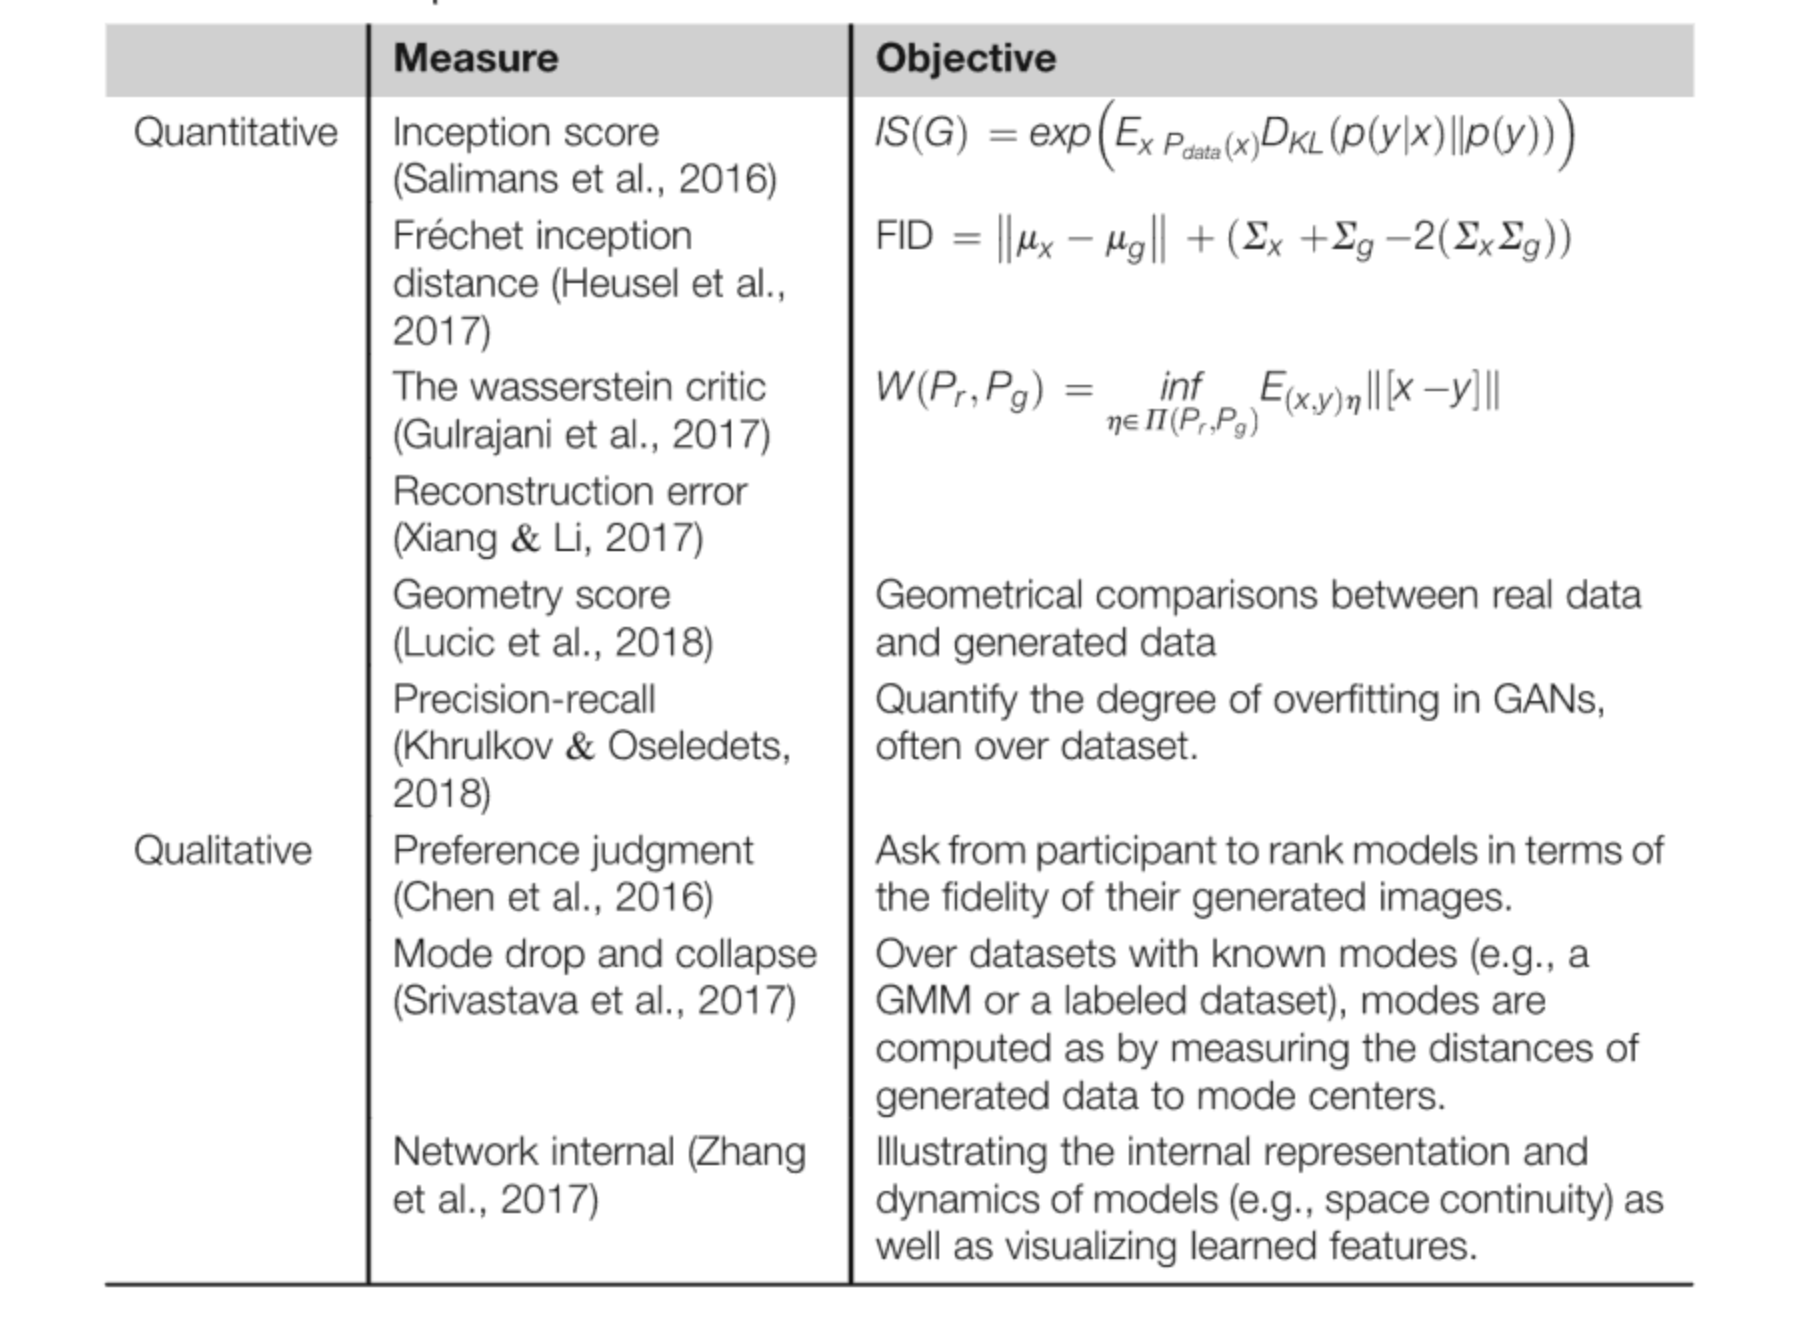
\includegraphics[width=8cm]{plots/evaluationGAN.png}
%        \centering \tiny{source: M. Rezaei (2020) }
%   \end{figure}
%   
%\end{frame}
%
%\begin{frame} {GAN Evaluation- Inception Score}
%\vspace{1mm}
%The inception score measures the quality of generated samples.
%\vspace{2mm}
%  \begin{itemize}
%   \item They used the Inception model (Szegedy et al., 2015)  trained on ImageNet
%   \item Given generated image $x$, assigned the label $y$ by model $p$:\\
%   $P(y|x)  \rightarrow $ low entropy (one class)
%   \item The distribution over all generated images should be spread (evaluating mode collapse) \\
%   $\int P(y|x = G(z)) dz \rightarrow $ high entropy (many classes)
%   \item The distribution over all generated images should be spread: 
%(evaluating mode collapse) \\
%$exp (E_x KL (p (y|x) || p(y)))$
%  \end{itemize}
%
%
%\end{frame}

%%%%%%%%%%%%%%%%%%%%%%%%%%%%%%%%%%%%%%%%%%%%%%%%%%%%%%%%%%%%%%%%%%
%%%%%%%%%%%%%%%%%%          REFERENCES          %%%%%%%%%%%%%%%%%%
%%%%%%%%%%%%%%%%%%%%%%%%%%%%%%%%%%%%%%%%%%%%%%%%%%%%%%%%%%%%%%%%%%
\begin{vbframe}
\frametitle{References}
\footnotesize{
\begin{thebibliography}{99}
% %%%%%%%%%%%%%%%%%%%%%%%%%%%%%%%%%%
% \bibitem[Zhang et al., 2017]{1} Han Zhang, Tao Xu, Hongsheng Li, Shaoting Zhang, Xiaogang Wang, Xiaolei Huang, Dimitris Metaxas (2017)
% \newblock StackGAN: Text to Photo-realistic Image Synthesis with Stacked Generative Adversarial Networks
% \newblock \emph{\url{https://arxiv.org/abs/1612.03242}}
% %%%%%%%%%%%%%%%%%%%%%%%%%%%%%%%%%%
% %%%%%%%%%%%%%%%%%%%%%%%%%%%%%%%%%
% \bibitem[Wang et al., 2017]{2} Ting-Chun Wang, Ming-Yu Liu, Jun-Yan Zhu, Andrew Tao, Jan Kautz, Bryan Catanzaro (2017)
% \newblock High-Resolution Image Synthesis and Semantic Manipulation with Conditional GANs
% \newblock \emph{\url{https://arxiv.org/abs/1711.11585}}
% %%%%%%%%%%%%%%%%%%%%%%%%%%%%%%%%%%
%%%%%%%%%%%%%%%%%%%%%%%%%%%%%%%%%
\bibitem[Goodfellow et al., 2014]{5} Ian J. Goodfellow, Jean Pouget-Abadie, Mehdi Mirza, Bing Xu, David Warde-Farley, Sherjil Ozair, Aaron Courville, Yoshua Bengio (2014)
\newblock Generative Adversarial Networks
\newblock \emph{\url{https://arxiv.org/abs/1406.2661}}
%%%%%%%%%%%%%%%%%%%%%%%%%%%%%%%%%%
%%%%%%%%%%%%%%%%%%%%%%%%%%%%%%%%%
\bibitem[Pascual et al., 2017]{6} Santiago Pascual, Antonio Bonafonte, Joan Serra (2017)
\newblock SEGAN: Speech Enhancement Generative Adversarial Network
\newblock \emph{\url{https://arxiv.org/abs/1703.09452}}
%%%%%%%%%%%%%%%%%%%%%%%%%%%%%%%%%%
%%%%%%%%%%%%%%%%%%%%%%%%%%%%%%%%%
\bibitem[Goodfellow, 2016]{7} Ian Goodfellow (2016)
\newblock NIPS 2016 Tutorial: Generative Adversarial Networks
\newblock \emph{\url{https://arxiv.org/abs/1701.00160}}
%%%%%%%%%%%%%%%%%%%%%%%%%%%%%%%%%%
%%%%%%%%%%%%%%%%%%%%%%%%%%%%%%%%%
\bibitem[Weng, 2017]{8} Lilian Weng (2017)
\newblock From GAN to WGAN
\newblock \emph{\url{https://lilianweng.github.io/lil-log/2017/08/20/from-GAN-to-WGAN.html}}
%%%%%%%%%%%%%%%%%%%%%%%%%%%%%%%%%%
%%%%%%%%%%%%%%%%%%%%%%%%%%%%%%%%%
\bibitem[Chang, 2016]{9} Mark Chang (2016)
\newblock Generative Adversarial Networks
\newblock \emph{\url{https://www.slideshare.net/ckmarkohchang/generative-adversarial-networks}}
%%%%%%%%%%%%%%%%%%%%%%%%%%%%%%%%%%
%%%%%%%%%%%%%%%%%%%%%%%%%%%%%%%%%
\bibitem[Theis et al., 2016]{10} Lucas Theis, Aaron van den Oord, Matthias Bethge (2016)
\newblock A note on the evaluation of generative models
\newblock \emph{\url{https://arxiv.org/abs/1511.01844}}
%%%%%%%%%%%%%%%%%%%%%%%%%%%%%%%%%%
%%%%%%%%%%%%%%%%%%%%%%%%%%%%%%%%%
\bibitem[Nibali, 2016]{11} Aiden Nibali (2016)
\newblock The GAN objective, from practice to theory and back again
\newblock \emph{\url{https://aiden.nibali.org/blog/2016-12-21-gan-objective/}}
%%%%%%%%%%%%%%%%%%%%%%%%%%%%%%%%%%
%%%%%%%%%%%%%%%%%%%%%%%%%%%%%%%%%
\bibitem[Mirza, 2014]{12} Mehdi Mirza, Simon Osindero (2014)
\newblock Conditional Generative Adversarial Nets
\newblock \emph{\url{https://arxiv.org/abs/1411.1784}}
%%%%%%%%%%%%%%%%%%%%%%%%%%%%%%%%%%
%%%%%%%%%%%%%%%%%%%%%%%%%%%%%%%%%
\bibitem[Isola et al., 2016]{13} Phillip Isola, Jun-Yan Zhu, Tinghui Zhou, Alexei A. Efros (2016)
\newblock Image-to-Image Translation with Conditional Adversarial Networks
\newblock \emph{\url{https://arxiv.org/abs/1611.07004}}
%%%%%%%%%%%%%%%%%%%%%%%%%%%%%%%%%%
%%%%%%%%%%%%%%%%%%%%%%%%%%%%%%%%%
\bibitem[Perarnau, 2017]{14} Guim Perarnau (2017)
\newblock Fantastic GANs and where to find them
\newblock \emph{\url{https://guimperarnau.com/blog/2017/03/Fantastic-GANs-and-where-to-find-them}}
%%%%%%%%%%%%%%%%%%%%%%%%%%%%%%%%%%
%%%%%%%%%%%%%%%%%%%%%%%%%%%%%%%%%


\end{thebibliography}
}
\end{vbframe}
%%%%%%%%%%%%%%%%%%%%%%%%%%%%%%%%%%%%%%%%%%%%%%%%%%%%%%%%%%%%%%%%%%
%%%%%%%%%%%%%%%%%%%%%%%%%%%%%%%%%%%%%%%%%%%%%%%%%%%%%%%%%%%%%%%%%%

\endlecture
\end{document}
